\documentclass[a4paper,11pt,twoside]{report}
\usepackage[utf8]{inputenc}
\usepackage[T1]{fontenc}
\usepackage{textcomp}
\usepackage{amsmath, amssymb}
\usepackage{hyperref}
\usepackage{listings}
\usepackage{xcolor}
\usepackage{bookmark}
\usepackage{authblk}
\usepackage{fancyhdr, blindtext}
\usepackage{algorithm}
\usepackage{algpseudocode}
\usepackage{mathpazo}
\usepackage{soul}

\pagestyle{fancy}
\fancyhf{}
\fancyhead[le]{\nouppercase{\rightmark}}
\fancyhead[re]{\thepage}
\fancyhead[RO]{\nouppercase{\leftmark}} % chapter
\fancyhead[LO]{\thepage}
\setlength{\headheight}{15pt}

\definecolor{codegreen}{rgb}{0,0.6,0}
\definecolor{codegray}{rgb}{0.5,0.5,0.5}
\definecolor{codepurple}{rgb}{0.58,0,0.82}
\definecolor{backcolour}{rgb}{0.98,0.98,0.92}

\hypersetup{
    colorlinks=true,
    linkcolor=blue,
    filecolor=magenta,      
    urlcolor=blue,
    % pdftitle={CLA Commentary},
    pdfpagemode=FullScreen,
    }

\urlstyle{same}

\lstdefinestyle{mystyle}{
    backgroundcolor=\color{backcolour},
    commentstyle=\color{codegreen},
    keywordstyle=\color{magenta},
    numberstyle=\tiny\color{codegray},
    stringstyle=\color{codepurple},
    basicstyle=\ttfamily\footnotesize,
    breakatwhitespace=false,
    breaklines=true,
    captionpos=b,
    keepspaces=true,
    numbersep=5pt,
    showspaces=false,
    showstringspaces=false,
    showtabs=false,
    tabsize=2
}

\lstset{style=mystyle}


\newenvironment{spmatrix}[1]
 {\def\mysubscript{#1}\mathop\bgroup\begin{pmatrix}}
 {\end{pmatrix}\egroup_{\textstyle\mathstrut\mysubscript}}
 
% figure support
\usepackage{import}
\usepackage{xifthen}
\usepackage{pdfpages}
\usepackage{transparent}
\usepackage{tikz}
\usetikzlibrary{calc}
\usepackage{float}
\usepackage{subcaption}
\usepackage[export]{adjustbox}
\newcommand{\incfig}[1]{%
  \def\svgwidth{\columnwidth}
  \import{./figures/}{#1.pdf_tex}
}
\newcommand{\checked}{\makebox[0pt][l]{$\square$}\raisebox{.15ex}{\hspace{0.1em}$\checkmark$}}

\tikzset{
    right angle quadrant/.code={
        \pgfmathsetmacro\quadranta{{1,1,-1,-1}[#1-1]}     % Arrays for selecting quadrant
        \pgfmathsetmacro\quadrantb{{1,-1,-1,1}[#1-1]}},
    right angle quadrant=1, % Make sure it is set, even if not called explicitly
    right angle length/.code={\def\rightanglelength{#1}},   % Length of symbol
    right angle length=2ex, % Make sure it is set...
    right angle symbol/.style n args={3}{
        insert path={
            let \p0 = ($(#1)!(#3)!(#2)$) in     % Intersection
                let \p1 = ($(\p0)!\quadranta*\rightanglelength!(#3)$), % Point on base line
                \p2 = ($(\p0)!\quadrantb*\rightanglelength!(#2)$) in % Point on perpendicular line
                let \p3 = ($(\p1)+(\p2)-(\p0)$) in  % Corner point of symbol
            (\p1) -- (\p3) -- (\p2)
        }
    }
}



\begin{document}
\title{MATH60024 \\ Computational Linear Algebra \\
Commentary Notes}
\date{Autumn 2021-2022}
\author{Feifan Fan}
\affil{\textit{based on lecture contents} 
\\ \textit{by Professor Colin Cotter}}




\maketitle
\chapter*{Declaration}
This so-called "commentary notes" is based on lecture notes of MATH60024, Computational Linear Algebra, which is led and lectured by Professor Colin Cotter. 
The original notes could be found \href{https://comp-lin-alg.github.io}{here}. I would refer it as "master notes" most of the time in the following commentary.

I wrote this set of notes to explain the important points in the master notes, making extra examples and detailed proofs about concepts and theorems which is not somehow vague, and give step-by-step instructions and hints for doing the \textbf{assessed} coding exercise.

Obviously I would not show you my code directly, since it is not good for you to practice and improve the coding skills, and not fair to my dedicated 30hr+ code implementation work last year.

However, my hints would be aimed at helping you have a deeper understanding of the problem description and knowledge itself, and also let you to understand the implementations from scratch (I hope so :-D).

There is no need to worry if you think you didn't do the \href{https://object-oriented-python.github.io}{Priciples of Programming} module in year 2. The module is beneficial but not necessary. What you need to do is just giving yourself enough coding practice via attempting the exercises in this module (and read my hints carefully if you get stuck!). Programming is the art of craftsmanship, and dedicated practice would lead you to perfection.


You might find that I would spend time in proving theorems, although this module is totally "computational". The reason I did this is just to make sure everything could be demonstrated clearly. If you are not happy with reading proofs, feel free to skip them!

This module would be a great adventure, hope you enjoy and have lots of fun in this journey!

\chapter*{Acknowledgements}
Firstly I want to thank Professor Colin Cotter for providing such a brilliant set of open-sourced master notes first.
Without his extraordinary work, I cannot digest the knowledge in such a quick and enjoyable way, and come up with the idea of writing these "commentary notes". 
I hope my work would help him and students studying this module in the following years.\smallskip

My parents are also in my first place to say thanks. They are always the people I could share my feelings and find help. Special thanks to my mom - who studied mathematics in uni and worked as a maths teacher, giving me the talent in particular linear algebra and statistics. She always encouraged me to embrace opportunity of explaining studying materials to my colleagues and friends - and that's why I decided to write this document.\smallskip

Thanks a lot to my friends Tiansheng, Kexin and Di (pronounced as \textbf{Dee}) being the first group of readers of the notes. Their participation of reading notes and using this as additional studying material in Autumn 2021 gives me extra motivation in studying ahead of the course schedule and finding a more clear way to deliver the contents in-person.\smallskip

I would also like to thank my two friends who motivated me to make more progress in completing the notes (and they might not realise that). They were struggling with notes with vague explanations and lack of mentioning programming skills in their year 2, and I would like to give them as the very first gift of their year 3 pathway at Imperial. Their enthusiasm for mathematics also gave me the opportunity to rethink about the module, and what would I expect in the material if I started this module again.\smallskip

This project-based module might be hard, intensive with workload and deadlines, and annoying if you cannot figure about either mathematics or programming part. However, I hope this supplementary material (and/or myself) could be the place that the readers always rely on, no matter how complex or annoying the problem they encountered is.\smallskip

With my work, I hope students not only remember this module because of the multiple intensive 3-day-limited courseworks and 1-less exam in the summer term, but also the fun of understanding the maths, using maths to implement functions, and utilising functions to solve mathematical/real-word problems.
\tableofcontents
\listoffigures

\chapter{Preliminaries}
\subsection*{Material Correspondence Table}
I reconstructed the original study material by dividing some parts into smaller sections to make a step-by-step approach of the content in the notes. \smallskip

\noindent If you want to see correspondence of the materials between the original and commentary notes, here is a table indicating the relations: \bigskip

\noindent 
\begin{tabular}{ll}
  Master Notes & Commentary Notes \\
  \hline \\
  1.1. Matrices, vectors and matrix-vector multiplication & Section 1.1 - 1.3 \\
  1.2. Range, nullspace and rank & Section 1.4 - 1.6 \\
  1.3. Invertibility and inverses & Section 1.7  \\
  1.4. Adjoints and Hermitian matrices & Section 1.8 \\
  1.5. Inner products and orthogonality & Section 1.9 \\
  1.6. Orthogonal components of a vector & Section 1.10\\
  1.7. Unitary matrices & Section 1.11  \\
  1.8. Vector norms & Section 1.9\\
  1.9. Projectors and projections &  Section 1.12 \\
  1.10. Constructing orthogonal projectors  & Section 1.13
  \end{tabular}
\newpage
\section{Matrix-Vector Multiplication}%
\textbf{This part might be too easy for most of you - but it would still give you intuition in the contents we would discuss later.}\medskip

\noindent Note that in this course we would discuss \textbf{vectors in \(\mathbb{C}^{n}\) rather than \(\mathbb{R}^{n}\)}, so some vector operations would be different from those you get used to. You would see the details as we going through the course.
\subsection*{Content Checklist}
\noindent In this section we would:
\begin{itemize}
  \item Recap on \textbf{Matrix-Vector multiplication formula}. 
  \item \textbf{Implement a Python function} for M-V multiplication.
\end{itemize}
\subsection*{Contents}
\begin{definition}[Matrix-Vector Multiplication]
  Suppose we are given that:
  \[
    x = \begin{pmatrix} x_1\\x_2\\ \vdots\\ x_n \end{pmatrix} \in \mathbb{C}^{n} \text{ and } 
      A = \begin{pmatrix} 
      a_{11} & a_{12} & \ldots & a_{1n} \\
    a_{21} & a_{22} & \ldots & a_{2n} \\ 
    \vdots & \vdots & \ddots & \vdots \\
    a_{m1} & a_{m2} & \ldots & a_{mn} \\  
    \end{pmatrix} \in \mathbb{C}^{m \times n}
  .\] 
  The problem asked to compute value of $b = Ax$ is called the \textbf{Matrix-Vector} multiplication problem, where
  \[
    b_i = \sum_{j = 1}^{n} a_{ij}x_j, \text{ where } i \in \{1, 2, 3 \ldots m\} 
    .\checked\] 
\end{definition}
This operation, or we say the map $x \to  Ax$ is indeed a linear map from $\mathbb{C}^{n} \to \mathbb{C}^{m}$. 
This should be really straightforward for you and I would skip the proof. \medskip

\noindent Now you can compute the \(i\)th entry \(b_i\) from the formula above. Consider how you normally compute the value of \(b\), and how to use this schema further to implement a python function. Try exercise 1.1 to see if you could convert the math to executable code.
\subsection*{Exercise 1.1: Basic M-V Multiplication}
\addcontentsline{toc}{subsection}{Exercise 1.1: Basic M-V Multiplication}
\begin{problem}
  Given matrix $A$ and vector $x$ as defined above, you need to implement a function \href{https://comp-lin-alg.github.io/cla_utils.html#cla_utils.exercises1.basic_matvec}{\texttt{exercises1.basic\_matvec()}}
under the \texttt{cla\_utils} package, which returns the matrix-vector product $b = Ax$.
\end{problem}
\noindent I would give you some instructions in this exercise:
\begin{enumerate}
  \item Clearly to compute value of \(b\)  we need to compute all \(m\)  entries \textbf{repeatedly}, just like what we normally do with paper and pens. So a \textbf{for} loop in the form \texttt{for i in range(m)} is required. In this loop, we compute \(b_i\) for each value of \(i\).
  \item To compute \(b_i\), we apply the formula with summation variable \(j\). You should see we need another \textbf{for} loop in the form \texttt{for j in range(n)} to compute \(b_i\)  , since \(j\) is changing from 1 to n in the formula. 
  \item When computing \(b_i\), what you need to do is just keep adding summation components, and finally store the value into your final \(b\). \checked
\end{enumerate}
The instructions should be clear enough for you to start the very first exercise. The most naive structure of code should be:
\begin{lstlisting}[language=Python]
import numpy as np
def basic_matvec(A, x):
    # Get the dimensions of A
    m, n = ...
    # Initialise vector b as a zero vector.
    b = np.zeros(n)
    for i in range(m):
        b_i = 0
        # Compute the value of b_i.
        for j in range(n):
            # Apply the basic formula in summation.
            b_i += ...
        # set the ith entry of b as b_i.
        b[i] = b_i
    return b
\end{lstlisting}
\textbf{Make sure your code implementation pass the provided test cases.}
\section{Column-Space Formulation}
\label{sec1.2}
In this section, we would give you an intuition to interpret matrix-vector multiplication as a linear combination of columns of $A$, with coefficients taken from the entries of $x$.
\subsection*{Content Checklist}
\noindent In this section we would:
\begin{itemize}
  \item Introduce the concept of \textbf{Column-Space Formulation}. 
  \item \textbf{Implement a Python function} for M-V multiplication with C-S Interpretation.
\end{itemize}
\subsection*{Contents}
\begin{definition}[Column-Space Formulation]
  Suppose we have matrix \(A\)  in the form
  \[
    A = \begin{pmatrix}
      a_1 & a_2 & \ldots & a_n
    \end{pmatrix}
  .\]
  The result of \(b = Ax\)  is a linear combination of columns of \(A\), \(a_i\)  with the entries of \(x\)  as coefficients. i.e.
  \[
    b = Ax =  \sum_{i=1}^{n} x_i a_i
  .\]
\end{definition}
\begin{explanation}
  We firstly ignore the special form of \(A\) with column notation, and use the basic M-V multiplication formula to expand \(b\):
  \[
b = \begin{pmatrix} a_{11}x_1 + a_{12}x_2 + \cdots + a_{1n}x_n \\  a_{21}x_1 + a_{22}x_2 + \cdots + a_{2n}x_n\\ \vdots\\a_{m1}x_1 + a_{m2}x_2 + \cdots + a_{mn}x_n \end{pmatrix}
\]
Indeed this is equivalent to
\[
b = x_1\begin{pmatrix} a_{11}\\ a_{21} \\ \vdots\\ a_{m1} \end{pmatrix} + x_2 
\begin{pmatrix} a_{12}\\ a_{22} \\ \vdots\\ a_{m2} \end{pmatrix} + \cdots + x_n 
\begin{pmatrix} a_{1n}\\ a_{2n} \\ \vdots\\ a_{mn} \end{pmatrix}
.\]
Then we apply the special column notation \(a_i = \begin{pmatrix} a_{1i} & a_{2i} & \ldots & a_{mi} \end{pmatrix}^{\top}\) and we should get
\[
  b = x_1a_1 + x_2a_2 + \cdots + x_na_n = \sum_{j=1}^{n} x_j a_j
.\]
with \(b\) as a linear combination of columns of \(A\) and entries of $x$. 
\end{explanation}

\begin{note}
  You could see now \(b\)  is spanned by columns of \(A\) , and that is why we called it Column-Space Formulation (or Interpretation).
\end{note}

\subsection*{Exercise 1.2: M-V Multiplication with C-S Formulation}%
\addcontentsline{toc}{subsection}{Exercise 1.2: M-V Multiplication with C-S Formulation}
\begin{problem}
  We were still considering to compute the value of \(b = Ax\), but now you are asked to implement a function \href{https://comp-lin-alg.github.io/cla_utils.html#cla_utils.exercises1.column_matvec}{\texttt{column\_matvec()}} with \textbf{exactly one loop} over entries of \(A\) (and \(x\)).
\end{problem}
\noindent You might find the column-space formulation we mentioned above is helpful for inplementation, i.e.:
\[
b = Ax =  \sum_{i=1}^{n} x_i a_i
.\]

\begin{hint} 
Here are several things also worth mentioning:

\begin{enumerate}
\item Since we are asked to use a \textbf{single loop} only, we could easily see that using the formula above with one $\Sigma$ sign would work. 
\item Then what you need to do is just add up the multiples of column vectors in the loop. Make sure you know how to get the \(i\)th column vector from \(A\)  in \texttt{numpy}. \checked
\end{enumerate}
\textbf{Make sure your implementation pass the provided test cases.}
\end{hint}

\section{Matrix-Matrix Multiplication}%
\label{sec1.3}
\subsection*{Content Checklist}
\noindent In this section we would:
\begin{itemize}
  \item Extend the multiplication formula for the \textbf{Matrix-Matrix} Case.
  \item Recap and extend the \textbf{outer} and \textbf{inner} product of vectors in \(\mathbb{C}^{m}\).
  \item Compare the \textbf{execution time} of M-V multiplication with \textbf{different implementations}.
\end{itemize}
\subsection*{Contents}
\begin{definition}[Matrix-Matrix Multiplication]
  Suppose we are given $A \in \mathbb{C}^{m \times l}m C \in \mathbb{C}^{l \times n}$, to compute matrix $B = AC$ we have:
  \[
    b_{ij} = \sum_{k = 1}^{l} a_{ik}c_{kj} 
  .\]  
\end{definition}
\begin{note}
  If we consider the relation between the \(i\)th column of \(B\) and \(C\), \(b_i\)  and \(c_i\), you would see
  \[
    b_i = Ac_i
  .\]
  which means the \textbf{\(i\)th column} of \(B\) is the \textbf{matrix-vector product} of A with the \textbf{\(i\)th column} of \(C\). This is very important for you when understanding the matrix factorisation algorithms in the following chapters. \checked
\end{note}
However, you might consider what would happen if two vector-like matrices multiply together, i.e. multiplication between \(m \times 1\) and \(1 \times  m\) matrices. Here we define the \textbf{outer product} for vectors to describe this operation:
\begin{definition}[Outer Products for Real Vectors]
  Suppose \(u, v \in \mathbb{R}^{m}\), the outer product between \(u\) and \(v\) is:
  \[
    uv^{\top} = \begin{pmatrix} 
      uv_1 & uv_2 & \dots & uv_m 
    \end{pmatrix} \in \mathbb{R}^{m\times m}
  .\]
\end{definition}
and we could extend this definition to \textbf{complex vectors}:
\begin{definition}[Outer Products for Complex Vectors]
  Suppose \(u, v \in \mathbb{C}^{m}\), the outer product between \(u\)  and \(v\)  is:
  \[
    uv^{*} = \begin{pmatrix} 
      u\overline{v_1} & u\overline{v_2} & \dots & u\overline{v_m}
    \end{pmatrix} \in \mathbb{C}^{m \times  m} 
  .\]
  where \(v^{*}\) is the complex conjugate of \(v^{\top}\).
\end{definition}     
The \(^{*}\) sign is also widely used in finding adjoints of complex matrices. We would discuss the properties further in \autoref{sec1.7}. \smallskip

\noindent And we have also defined \textbf{inner product} which gives out a scalar:
\begin{definition}[Inner Products for Complex Vectors]
  Suppose \(u, v \in \mathbb{C}^{m}\), the inner product between \(u\)  and \(v\)  is:
  \[
    u^{*}v = \sum_{i=1}^{m} \overline{u_i}v_i \in \mathbb{C}
  .\] 
\end{definition}   
\begin{property}
  The inner product is bilinear.
\end{property}
The concept of inner product is strongly related to the orthogonality and norm of vectors. We would discuss the concepts further in \autoref{sec1.8}. \checked
\subsection*{Exercise 1.3: Execution Time Comparison}%
\addcontentsline{toc}{subsection}{Exercise 1.3: Execution Time Comparison}
You don't need to implement anything in this exercise, but just run several lines of code in your terminal. \textbf{This exercise is not assessed.}
\begin{problem}
Now you have two equivalent implementations of matrix-vector multiplication, and we want to see how fast these two and the default \texttt{numpy} implementation could handle the matrix-vector problem. 

\noindent Use the pre-defined function $\texttt{time\_matvecs()}$ to see the execution time among the following implementations:
\begin{lstlisting}
> basic_matvec(A0, x0) # double-nested loop implementation

> column_matvec(A0, x0) # single loop implementation

> A0 @ x0 # using @ ("at" sign) as matmul operator in numpy
\end{lstlisting}
\end{problem}
\subsubsection*{Efficiency Measuring}
Run the following code in your terminal and you could see:
\begin{lstlisting}
>>> import cla_utils
>>> cla_utils.time_matvecs()
Timing for basic_matvec
0.09208189499999975
Timing for column_matvec
0.002095079000000055
Timing for numpy matvec
0.00014622799999841618
\end{lstlisting}
All methods should be equivalent, but as for the execution time:
\[
\texttt{basic} \gg \texttt{column-space} \gg \texttt{numpy implementation}
.\]
This is because \texttt{numpy} optimised the efficiency in general numerical operations. Therefore, in this course you are always recommended to use basic \texttt{numpy} functions other than your own implementation, except the case you are not allowed to use some functions e.g. \texttt{np.linalg.qr()}. \checked
\section{Range of a Matrix}%
\label{sec1.4}
\subsection*{Content Checklist}
\noindent In this section we would:
\begin{itemize}
  \item Introduce the concept of \textbf{range}.
  \item Relate range of matrix to the \textbf{span} of column vectors. 
\end{itemize}
\subsection*{Contents}
\begin{definition}[Range of a Matrix]
  Suppose \(A \in \mathbb{C}^{m \times n}\), the range of \(A\) is defined as:
  \[
  \text{range}(A) = \{a : \exists x \in \mathbb{C}^{n}, Ax = a \}
  .\checked\]
\end{definition}
One interesting conclusion about range is:
\begin{prop}[range equals to span of column vectors]
  \[
    \text{range}(A) = \text{span}(a_1, \cdots, a_n)
  .\] 
  i.e. range($A$) is the vector space spanned by the columns of $A$.
\end{prop}
This is obvious to see. Let me explain it a little bit. 

\noindent Since any vector \(a \in\) range\((A)\)  is in the form \(Ax\), i.e. any vector in range of \(A\)  is a linear combination of column vectors of \(A\), and it would also be in the vector space spanned by column vectors.

\noindent Also, since any vector in span of column vectors is a linear combination of the columns, it should also be an element of range($A$), job done. \checked


\section{Null Space and Rank of a Matrix}%
\label{sec1.5}
\subsection*{Content Checklist}
\noindent In this section we would:
\begin{itemize}
  \item Introduce the concept of null space and rank.
  \item Learn to construct a \textbf{rank-2 matrix} with python.
\end{itemize}
\subsection*{Contents}
\begin{definition}[Null Space of a Matrix]
  Suppose \(A \in \mathbb{C}^{m \times n}\), the null space of \(A\) is defined as:
  \[
    \text{null}(A) = \{x \in \mathbb{C}^{n}: Ax = 0\} 
  .\]
\end{definition}

\begin{definition}[Rank of a Matrix]
  \[
  \text{rank}(A) = \text{dim}(\text{span}(a_1, a_2, \cdots, a_n)) = \text{dim}(\text{range}(A))
\]
where \(a_i\)  column vectors. 
\end{definition}
\begin{property}
  \(\forall A \in \mathbb{C}^{m \times n}\), rank\((A) \leq \min(m, n)\).
\end{property}
\begin{definition}[Full Rank]
  Suppose \(A \in \mathbb{C}^{m \times n}\), if 
  \[
    \text{rank}(A) = \min(m, n)
  \]
  we say \(A\) has a full rank. \checked
\end{definition}

\subsection*{Exercise 1.11: Construct a Rank-2 Matrix}%
\addcontentsline{toc}{subsection}{Exercise 1.11: Construct a Rank-2 Matrix}
\begin{problem}
  Given that we have $u_1, u_2 \in \mathbb{C}^{m}$ and $v_1, v_2 \in \mathbb{C}^{n}$, we want to construct a rank-2 matrix $A = u_1v_1^{*} + u_2v_2^{*}$. However, from the given code and the specification, we need to implement a function \href{https://comp-lin-alg.github.io/cla_utils.html#cla_utils.exercises1.rank2}{\texttt{exercises1.rank2()}} returning matrix  $A$ as a product of two other matrices $B$ and $C$.
\end{problem}
\begin{hint}
  We need to consider the following two questions:
\end{hint}
\begin{itemize}
  \item How to expand $A$ from outer products?
  \item Can you find the relation between columns of \(A\), \(u\) and \(v\)?
\end{itemize}
Pause at here for a moment to think about these two questions. Feel free to read the answers in the next page if you get confused.
\newpage

\noindent Here we consider the $A$ as a summation of two matrices first:
\[
A = u_1v_1^{*} + u_2v_2^{*}
\]
where
\[
  u_1v_1^{*} = \begin{pmatrix} v_{11}^{*}u_1 & v_{12}^{*}u_1 & \cdots & v_{1n}^{*}u_1 \end{pmatrix} 
\]
and
\[
  u_2v_2^{*} = \begin{pmatrix} v_{21}^{*}u_2 & v_{22}^{*}u_2 & \cdots & v_{2n}^{*}u_2 \end{pmatrix} 
.\] 
Therefore, $A$ could be written in the sum:
\[
  A = u_1v_1^{*} + u_2v_2^{*} = \begin{pmatrix} v_{11}^{*}u_1 + v_{21}^{*}u_2 & v_{12}^{*}u_1 + v_{22}^{*}u_2 & \cdots & v_{1n}^{*}u_1 + v_{2n}^{*}u_2 \end{pmatrix} 
\]
with
\[
  a_{i} = v_{1i}^{*}u_1 + v_{2i}^{*}u_2 = \begin{pmatrix} u_1 & u_2 \end{pmatrix} \begin{pmatrix} v_{1i}^{*}\\ v_{2i}^{*} \end{pmatrix}
.\] 
To generalize this, we could now write $A$ in terms of a product of two matrices:
\[
A = \begin{pmatrix} u_1 & u_2 \end{pmatrix} \begin{pmatrix} v_{1}^{*}\\ v_{2}^{*} \end{pmatrix}   = \begin{pmatrix} u_1 & u_2 \end{pmatrix} \begin{pmatrix} v_{1}^{*} & v_{2}^{*} \end{pmatrix}^{\top}
.\]
So our first job has been done, now it is your time for implementation. \medskip

\noindent 
\textbf{Remember to check your implementation pass the provided test cases.}
\subsubsection*{Analysis}
Now let us talk about the rank of $A$, we claim the rank is necessarily 2.
Recall the result of $A$ we have found with column-space formulation: 
\[
A = u_1v_1^{*} + u_2v_2^{*} = \begin{pmatrix} v_{11}^{*}u_1 + v_{21}^{*}u_2 & v_{12}^{*}u_1 + v_{22}^{*}u_2 & \cdots & v_{1n}^{*}u_1 + v_{2n}^{*}u_2 \end{pmatrix} 
.\]
We could see that, every column of $A$ is a linear combination of $u_1$ and $u_2$, assume that they are linearly independent. Therefore, when we are talking about the range of $A$, it should be a vector space spanned by $u_1$ and $u_2$ and the dimension of the space should be 2. \textbf{i.e. the rank is 2 obviously.} \checked

\section{Invertibility and inverses}%
\label{sec1.6}
The idea and properties related to invertibility and inverses should be quite familiar, I would not talk about the definitions here. 
\subsection*{Content Checklist}
What I want to focus here is:
\begin{itemize}
  \item Relate finding the inverse to change of basis
  \item Coding exercise
\end{itemize}

\section*{Contents}
Consider the matrix-vector equation \(Ax = b\), assume \(A\) is invertible:
\begin{itemize}
  \item From entries of b, we could see the basis coefficients in the canonical basis $\{e_i\}$. 
  \item From the column-space formulation, we could see \(b\) is also a linear combination of columns of \(A\), with entries of \(x\) as basis coefficients and \(\{a_i\}\)  as basis. 
  \item Therefore, if we find \(x\), we could find a change of basis of \(b\)  from canonical basis to column basis \(\{a_i\}\).
  \item Since \(x = A^{-1}b\), we need to find \(A^{-1}\) to solve \(x\). Therefore we could say finding the inverse of matrix \(A\) can be seen as a change of basis.
\end{itemize}
This might not be relevant to the following exercise, but it would be helpful when you understand orthogonal projectors. \checked
\subsection*{Exercise 1.13: Find the inverse of a given matrix}%
\addcontentsline{toc}{subsection}{Exercise 1.13: Find the inverse of a given matrix}
\begin{problem}
  Given that a square matrix $A = I_m + uv^{*} \in \mathbb{C}^{m \times m}$, where $u, v \in \mathbb{C}^{m}$. Suppose we could find the inverse $A'$ written in  $A' = I_m + \alpha uv^{*}$, determine the value of $\alpha$ and implement the function \href{https://comp-lin-alg.github.io/cla_utils.html#cla_utils.exercises1.rank1pert_inv}{\texttt{rank1pert\_inv()}} to return the inverse matrix $A'$. \medskip
\end{problem}

\noindent Pause at here for a moment to think about writing value of \(\alpha\) in terms of \(u\) and \(v\). Feel free to read the answers in the next page if you get confused.
\newpage
\subsubsection*{What to do}
\noindent So we try to determine the value of $\alpha$ first:
\begin{itemize}
  \item Given that $A A^{-1} = I_m$:
    \[
      A A^{-1} = (I_m + u v^{*})(I_m + \alpha u v^{*}) = I_m + uv^{*} + \alpha uv^{*} + \alpha u v^{*}uv^{*} = I_m
    .\]
  \item Since the inner product, $v^{*}u$ is a scalar, then we could have:
    \[
      uv^{*} + \alpha uv^{*} + \alpha (v^{*}u)uv^{*} = 0_{m \times m} \implies (1 + \alpha + \alpha v^{*}u)uv^{*} = 0_{m \times m}
    .\]
  \item Therefore, we have:
    \[
    \alpha (1 + v^{*}u) = -1 \implies \alpha = -\frac{1}{1 + v^{*}u}
    \]
    and
    \[
    A^{-1} = I_m -\frac{1}{1 + v^{*}u} uv^{*}
    \]
    whenever $A$ is invertible.
\end{itemize}
So the code implementation for you should be very simple. \checked \medskip

\noindent \textbf{Check your implementation pass the provided test cases.}
\subsubsection*{Efficiency Measuring (Non-assessed part for this exercise)}
To measure the time taken for computing inverse of this implementation, and compare it with the built-in numpy implementation (just like what we did for timing the matrix-vector multiplication), I add the following code:
\lstinputlisting[language=Python, firstline=65, lastline=77]{./python/exercise1.py}
with pre-defined \texttt{u0}, \texttt{v0}, and the output shows that:
\begin{lstlisting}
>>> import cla_utils
>>> cla_utils.time_matinvs()
Timing for basic_matinv
0.0013024520000044504
Timing for numpy matinv
0.005589449000012792
\end{lstlisting}

\noindent We could see that the numpy implementation is slower. The reason of this output is that, unlike our implementation, the numpy implementation didn't take the advantage of structure of \(A\) - a rank-2 matrix constructed via \(u\) and \(v\), therefore, the complexity using numpy is greater than our implementation and the time taken is indeed longer.

\section{Adjoints and Hermitian Matrices}%
\label{sec1.7}
\subsection*{Content Checklist}
\noindent In this section we would:
\begin{itemize}
  \item Introduce the concept of Matrix Adjoints and Hermitian Matrices.
  \item Coding Exercise with a Hermitian matrix.
\end{itemize}
\subsection*{Contents}
\begin{definition}[Adjoints of Matrices]
  Suppose \(A \in \mathbb{C}^{m \times n}\), the adjoint (or Hermitian conjugate) \(A^{*} \in \mathbb{C}^{n \times m}\) is defined as:
  \[
    a^{*}_{ij} = \overline{a_{ji}}
  .\]
  which is equivalent to
  \[
    A^{*} = \overline{A^{\top}}
  .\]
\end{definition}
\begin{definition}[Hermitian Matrices]
  \[
    A^{*} = A \Rightarrow A \text{ Hermitian}  
  .\]
\end{definition}
\begin{property}
  \[ 
  (AB)^{*} = B^{*}A^{*}, A \in \mathbb{C}^{m \times n}, B \in \mathbb{C}^{n \times l}
.\] 
\end{property}
Feel free to prove this property.
And then we could look at the following exercise implementing the required function \href{https://comp-lin-alg.github.io/cla_utils.html#cla_utils.exercises1.ABiC}{\texttt{exercises1.ABiC()}}. \checked
\subsection*{Exercise 1.16: Hermitian Matrices and Multiplication}%
\addcontentsline{toc}{subsection}{Exercise 1.16: Hermitian Matrices and Multiplication}
This exercises have several mini-questions for us to solve. The first part is mainly about proof with hermitian matrices, and the function implementation part is about the application. Let's see the proof exercise first.

\subsubsection*{Task 1}%

\noindent Given that $A = B + iC \in \mathbb{C}^{m \times m}$ where $B, C$ are both real matrices with compatible dimensions, and  $A$ is hermitian, show that:
\[
  B = B^{\top} \text{ and } C = -C^{\top}
.\]
\begin{proof}
  Your work (but not assessed).
\end{proof}
\subsubsection*{Task 2}%
We required to compute the real and imaginary part of the matrix multiplication product $z = Ax$, where  $A$ is defined above. To save memory, the function would not accept the contents of $A$ as an argument, but a modified matrix $\hat{A}$, where
\[
\hat{A}_{ij} = \left\{
  \begin{array}{l}
  B_{ij} \text{ where } i \ge j \\
  C_{ij} \text{ where } i < j.
  \end{array}
\right.
.\] 
Therefore, given a matrix $\hat{A}$ and $x_r, x_i$ where  $x = x_r + ix_i$, we need to implement the function \href{https://comp-lin-alg.github.io/cla_utils.html#cla_utils.exercises1.ABiC}{\texttt{exercises1.ABiC()}} to get the real and imaginary parts of \(z = Ax\). Note that all your matrix-vector multiplication should be done via column-space formulation. \medskip

\noindent Pause at here for a moment to think about your implementation step by step. Feel free to read the instructions in the next page if you get confused.
\newpage
\subsubsection*{What to do}
\begin{enumerate}
\item Since we don't have contents of $A = B + iC$ as required, we could firstly try to get contents in $B$ and $C$ from $\hat{A}$.
\item The contents in $\hat{A}$ should look like this:
  \[
    \hat{A} = \begin{pmatrix} 
      b_{11} & c_{12} & c_{13} & \ldots & c_{1m} \\
      b_{21} & b_{22} & c_{23} & \ldots & c_{2m} \\
      b_{31} & b_{32} & b_{33} & \ldots & c_{3m} \\
      \vdots & \vdots & \vdots & \ddots & \vdots \\ 
      b_{m1} & b_{m2} & b_{m3} & \ldots & b_{mm}
    \end{pmatrix} 
  .\]
  So what we could do is to extract the lower-triangular part of $B$ and upper-triangular part of $C$ from $\hat{A}$, by using \texttt{np.triu()} and \texttt{np.tril()}, and then get the full form of $B$ and  $C$ by transposition.
 \item After having $B$ and $C$, we could simply calculate the value of  $z = Ax$:
    \[
      z = Ax = (B + iC)(x_r + ix_i) = (Bx_r - Cx_i) + i(Bx_i + Cx_r)
   \]
   where $z_r$ and $z_i$ could be easily seen. \checked
\end{enumerate}
\textbf{Remember to check your implementation pass the provided test cases.}
\newpage
\section{Inner Products, Orthogonality and Vector Norms}%
\label{sec1.8}
The idea of these concepts are very simple but they are extremely important in computational linear algebra. Here I would just focus on definitions to give you an insight.
\subsection*{Contents}
We have seen the definition of inner product in \autoref{sec1.3}, and the definition of 2-norm is based on that:
\begin{definition}[2-norm]
  Suppose \(x \in \mathbb{C}^{m}\), the 2-norm of \(x\) is defined as:
  \[
    \|x\| = \sqrt{\sum_{i=1}^{m} |x_i|^2} = \sqrt{x^{*}x}
  .\]
\end{definition}
And orthogonality is based on inner product and 2-norm:
\begin{definition}[Orthogonality]
  Suppose \(x, y \in \mathbb{C}^{m}\), we say \(x\) and \(y\) are orthogonal if
  \[
    x^{*}y = 0
  .\]
  Similarly two sets \(X, Y\) are orthogonal if
  \[
    \forall x \in X, y \in Y, x^{*}y = 0
  .\]
  And a set \(S\) is orthogonal itself if
  \[
    \forall x, y \in S,  x^{*}y = 0
  .\]
  A set \(S\) is orthonormal if \(S\) is orthogonal and \(\|x\| = 1 \forall x \in S\).   
\end{definition}
There are also definitions and properties about general norms and weighted norms mentioned in the original notes, but they are not quite relevant to the study material so I won't mention them here. \checked
\bigskip

\begin{center}
  \textit{\large End of Week 1}
\end{center}
% \newpage
% \section{Orthogonal Components of a Vector}%
% Given that we have a orthonormal set of vectors $S = \{q_1, q_2, \ldots, q_n\} $ where $q_i \in \mathbb{C}^{m}$, and for any vector $v \in \mathbb{C}^{m}$, we have:
% \[
%   v = r + \sum_{i=1}^{n} (q_iq_i^{*})v
% .\] 
% More specifically, it also shows that:
% \begin{itemize}
%   \item Given that we have an orthonormal set(basis) $S$, we could always split this vector to a linear combination of vectors in the orthonormal set, and a secret vector $r$. 
%   \item This secret vector $r$ orthogonal to any element in $S$.
%   \item So if we add $r$ to $S$ and gives out a new set $S'$, the newly formed set is still necessarily an orthonormal basis.
%   \item Can we use this idea in finding an orthonormal basis from any basis?
% \end{itemize}
% We would discuss this later in next chapter for $QR$ decomposition.
% \subsection*{Exercise 1.20: Orthonormal Decomposition of Vectors}
% \addcontentsline{toc}{subsection}{Exercise 1.20: Orthonormal Decomposition of Vectors}
% \subsubsection*{Problem Description}%
% Given a vector $v$ and an orthonormal set $Q$, we were asked to write $v$ as a sum of linear combination of elements in $Q$ \textbf{and} the residual vector $r$.

% \medskip
% \noindent The function \href{https://comp-lin-alg.github.io/cla_utils.html#cla_utils.exercises2.orthog_cpts}{\texttt{exercises2.orthog\_cpts()}} would do this work. It returns the coefficients $u$ in the linear combination, and the residual vector $r$. Your work is to implement this function.\subsubsection*{What to do}%
% \begin{enumerate}
% \item Recall that
%   \[
%     v = r + \sum_{i=1}^{n} (q^{*}_i v)q_i
%   .\]
%   We know that the coefficients $u_i$ comes from the inner product between $q_i$ and $v$ where $u_i = q^{*}_iv$.
% \item And what we need to do is just keep subtracting compoents of $q_i$ from $v$ (should be $u_iq_i$), until all orthogonal components are removed from  $v$, then we would get our  $r$.
% \item Think about it: can you get \(u, r\) without using loops? (You might use matrix multiplications, i.e. "vectorized" operations instead.)
% \item Note that implementations with \textbf{too many loops} may get your \textbf{mark down} during marking process. Sometimes using only one loop might be counted as "too much" as well.
% \end{enumerate} 
% \textbf{Remember to check your implementation pass the provided test cases.}
% \section{Unitary Matrices}%
% The definition, theorem and proof stated in the master notes in this section is clear enough, and I would like to emphasize one useful trick dealing with unitary matrices:
% \[
% Q \text{ is unitary } \iff Q^{*} = Q^{-1} \iff I = Q^{*}Q 
% .\] 
% and $Q^{*} = Q^{-1}$ could be interpreted as a change of orthogonal basis.
% \subsection*{Exercise 1.23: Solve the System $Qx=b$}
% \addcontentsline{toc}{subsection}{Exercise 1.23: Solve the System $Qx=b$ with Unitary Matrices}
% \subsubsection*{Problem Description}%
% Given a square \textbf{unitary} matrix $Q$ and a vector $b$, find the vector $x$ satisfies $Qx = b$ without using inverses of $Q$ in the implementation of \href{https://comp-lin-alg.github.io/cla_utils.html#cla_utils.exercises2.solveQ}{\texttt{solveQ()}}.

% \subsubsection*{What to do}%
% \begin{enumerate}
% \item Since we are not allowed to use inverses, and $Q$ is unitary, as we stated above, we could replace $Q^{-1}$ by $Q^{*}$ then $x = Q^{-1}b = Q^{*}b$.
% \item Then $Q^{*}$ could be easily represented as the combination of transposing the conjugate of matrix $Q$ via \texttt{numpy} operations.

% (Hint: try to consider \texttt{numpy.conj()} and \texttt{Q.T} as transpose of \texttt{Q}).
% \item Then we could simply get $x = Q^{*}b$ and implement the function.
% \end{enumerate}
% \textbf{Remember to check your implementation pass the provided test cases.}

% \subsubsection*{Efficiency Measuring (Non-assessed part for this exercise)}%
% To test the performance of function efficiency for random matrices with different sizes (compared with the general purpose \texttt{numpy.linalg.solve()}), we have the following code:
% \lstinputlisting[language=Python, firstline=17, lastline=31]{./python/exercise2.py}
% Here I pass an \texttt{lambda} (i.e. a "function call" with explicit arguments \texttt{Q} and \texttt{b}) to the \texttt{timeit.Timer} constructor rather than an pre-defined helper (timeable) function for code simplicity, and I can also pass variables to either \texttt{solveQ()} and \texttt{numpy.linalg.solve()} as I want.

% \medskip
% \noindent Since we use adjoint matrices rather than inverses, which reduces a certain amount of operations in finding inverses, so I would expect \texttt{solveQ()} would take less time than general purpose \texttt{solve()}. And the python console gives me the following result:

% \bigskip
% \begin{lstlisting}
% >>> import cla_utils
% >>> cla_utils.time_solveQ()
% --- Input matrix size n = 100 ---
% Timing for solveQ
% 0.00011220100000031152
% Timing for general purpose solve
% 0.0003564039999996993
% --- End for testing matrix with n = 100 ---
% --- Input matrix size n = 200 ---
% Timing for solveQ
% 0.00024624399999950697
% Timing for general purpose solve
% 0.0006074579999992835
% --- End for testing matrix with n = 200 ---
% --- Input matrix size n = 400 ---
% Timing for solveQ
% 0.0007872969999986879
% Timing for general purpose solve
% 0.002527909000001216
% --- End for testing matrix with n = 400 ---
% \end{lstlisting}
% We could easily see that our implementation is more efficient than the general purpose \texttt{solve()}, given that the matrix is unitary.

% \medskip
% \noindent Note: The explanation of vector norms in \href{https://comp-lin-alg.github.io/L1_preliminaries.html#vector-norms}{master notes 1.8} is clear enough so I would not cover this in my commentary.

% \section{Projectors and Projections}%
% The concept of projector is self-intuitive, but the relations between projector $P$ and its complementary projector are still worth mentioning.

% \medskip
% \noindent Let's consider a projector $P$ first:
% \begin{itemize}
%   \item Suppose $\exists x: Px=v$, i.e. $v \in \text{range}(P)$, we could see that:
%     \[
%       Pv = P(Px) = P^2x = Px = v
%     .\]
%     we could see projector $P$ doesn't change vectors in its range. (see \autoref{inrange}).
%   \item Suppose $v \not\in \text{range}(P)$, considering the vector $Pv - v$:
%      \[
%        P(Pv - v) = P^2v - Pv = Pv - Pv = 0
%     .\]
%     Here we could say $Pv - v$ is the nullspace of $P$, shown in \autoref{outrange}.
%   \begin{figure}[H]
%     \centering
%   \captionsetup[subfigure]{justification=centering}
%   \begin{subfigure}[b]{0.45\textwidth}
%     \centering
%     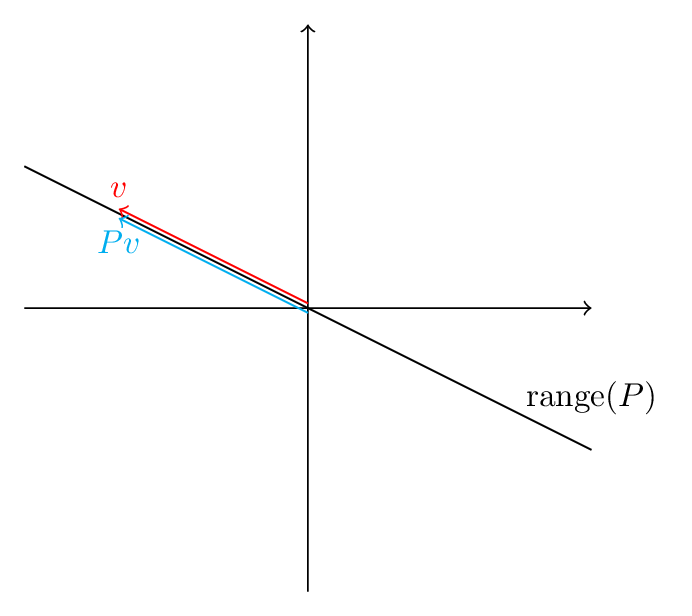
\includegraphics[width=\textwidth]{imgs/inline.png}
%     \caption{$v \in \text{range}(P)$}%
%     \label{inrange}
%     \end{subfigure}
%     \hfill
%     \begin{subfigure}[b]{0.5\textwidth}
%       \centering
%       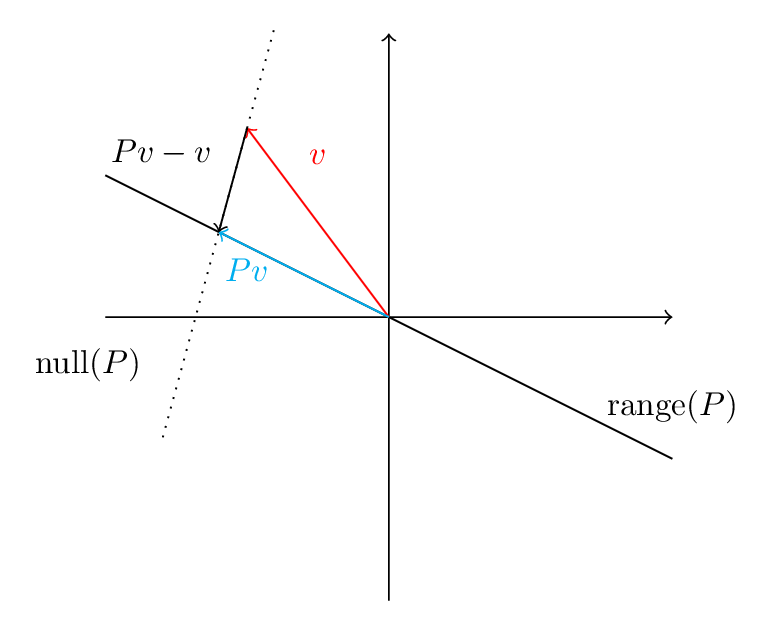
\includegraphics[width=\textwidth]{imgs/outrange.png}
%       \caption{$v \notin \text{range}(P)$}
%       \label{outrange}
%     \end{subfigure}
%     \caption{Projecting $v$ with projector $P$}
%   \end{figure}
% \end{itemize}
% Then consider the \textbf{complementary projector} $I - P$:
% \begin{itemize}
%   \item Obviously it's a projector as well. i.e. $(I - P)^2 = I - P$, and simply
%     \[
%       Pu = 0 \implies (I - P)u = u - Pu = u
%     .\]
%   \item The proposition above shows that, if a vector $u \in \text{null}(P)$, it is in $\text{range}(I - P)$. To generalize this, we have:
%     \[
%       [\forall u \in \text{null}(P) \implies \text{range}(I - P)] \implies
%     \]
%     \[
%       \text{null}(P) \subseteq \text{range}(I - P)
%     .\] 
%     In other words, the nullspace of $P$ is contained in the range of $I - P$.
%   \item Suppose there exists an vector $v \in \text{range}(I - P)$, in other words
%     \[
%       \exists w \in \mathbb{C}^{m}: v = (I - P)w = w - Pw
%     .\]
%   \item Then it shows that
%     \[
%       Pv = P(w - Pw) = Pw - P^2w = Pw - Pw = 0
%     .\] 
%   \item So indeed $v \in \text{null}(P)$, in this direction we could have:
%     \[
%       [v \in \text{range}(I - P) \implies v \in \text{null}(P)] \implies
%     \]
%     \[
%       \text{range}(I - P) \subseteq \text{null}(P)
%     .\]
%     \item And this leads to the result
%       \[
%         \text{null}(P) = \text{range}(I - P)
%       .\]
%       similarly
%       \[
%         \text{null}(I - P) = \text{range}(P)
%       .\] 
% \end{itemize}
% Important things for projector $P$: 
% \begin{itemize}
% \item  It separates  $\mathbb{C}^{m}$ into two spaces, range($P$) and null($P$), where 
%   \[
%   \text{range}(P) \cap \text{null}(P) = \{\textbf{0}\}
%   .\] 
%   The reason of why the intersection contains $\textbf{0}$ only is that, considering the two sets $\text{null}(P)$ and $\text{null}(I - P)$, the only common element is $\textbf{0}$. That is because any vector $v$ in both sets satisfies $v = v - Pv = (I - P)v = 0$. And since we know $\text{null}(I - P) = \text{range}(P)$, the results could be shown as stated above. 

% \item Conversely, if there exists two subspaces $S_1$ and $S_2$ of $\mathbb{C}^{m}$, where $S_1 \cap S_2 = \{\textbf{0}\}$, there exists a projector $P$ whose range is $S_1$ and nullspace is $S_2$.
% \end{itemize}
%   \subsubsection*{Proof}%
% \begin{itemize}
%   \item The proposition above states that, any vector in $\mathbb{C}^{m}$ could be split into two components, in subspaces $S_1$ and $S_2$ respectively.
%   \item Therefore, to prove this proposition, we could simplify this problem to the following proposition:
%     \[
%     \text{Given that } S_1 \cap S_2 = \{0\}, \forall v \in \mathbb{C}^{m}, \text{ find } v_1 \in S_1, v_2 \in S_2: v_1 + v_2 = v 
%     .\]
%     where the projection $Pv$ gives $v_1$ and the complementary projection $(I - P)v$ would gives $v_2$.
%   \item Obviously we could find the vector pair, since these two subspaces are distinct. But is the vector pair $(v_1, v_2)$ unique?
%   \item Suppose there exists another vector pair $(v_1', v_2') \in S_1 \times S_2$ which satisfies the conditions above, where clearly $v_i \neq v_i'$ and:
%     \[
%       \begin{array}{l}
%       v_1 + v_2 = v \\
%       v_1' + v_2' = v
%       \end{array}
%     .\] 
% \item Subtract the first equation by the second, and we get:
%   \[
%     (v_1 - v_1') + (v_2  - v_2') = \textbf{0} 
%   .\] 
% \item Say $v_1'' = v_1 - v_1'$ and $v_2'' = v_2 - v_2'$, and we could clearly see $v_i'' \in S_i$ due to the properties of subspaces. And we could get:
%   \[
%   v_1'' + v_2'' = \textbf{0} \implies v_1'' = -v_2''
%   .\]
%  \item We know that the subspace preserves scalar multiplication, therefore, we could see $v_1''$ is in $S_2$ and  $v_2''$ is in $S_1$ as well.
%   \item In this case, we know that $v_1'', v_2''$ are both in $S_1, S_2$. So we could interpret $v_1'', v_2'' \in S_1 \cap S_2 = \{\textbf{0}\} $.
%   \item Then obviously $v_1'' = v_2'' = \textbf{0}$, and
%     \[
%       \begin{array}{l}
%       v_1'' = v_1 - v_1' = \textbf{0} \\
%       v_2'' = v_2 - v_2' = \textbf{0} \\
%       \end{array}
%     \implies 
%       \begin{array}{l}
%       v_1 = v_1' \\
%       v_2 = v_2'
%       \end{array}
%     .\]
%     which contradicts our assumption $v_i \neq v_i'$, so the vector pair $(v_1, v_2)$ should be unique.
%     \item Therefore, we could find a unique decomposition of $v$ into two components $v_1, v_2$ in  $S_1$ and $S_2$. 
%     \item Since we take $v$ arbitrarily, and the components  $v_1, v_2$ in corresponding subspaces $S_1, S_2$ could be written as $Pv$ and  $(I - P)v$ for all chosen $v$, (which are both \textbf{bijection}). So we could say there exists a projector  $P$ such that range$(P) = S_1$ and null$(P) = S_2$.
% \end{itemize}


% \section{Orthogonal Projectors and Construction}%
% We have known the definition of projectors, but how about the orthogonal projectors? The definition states that a projector $P$ is orthogonal if:
% \[
% \forall v \in \mathbb{C}^{m}, (Pv)^{*}(Pv - v) = 0
% .\] 
% This definition might still be too abstract, so we put the definition into the following \autoref{orthogproj}:
%   \begin{figure}[H]
%     \centering
%     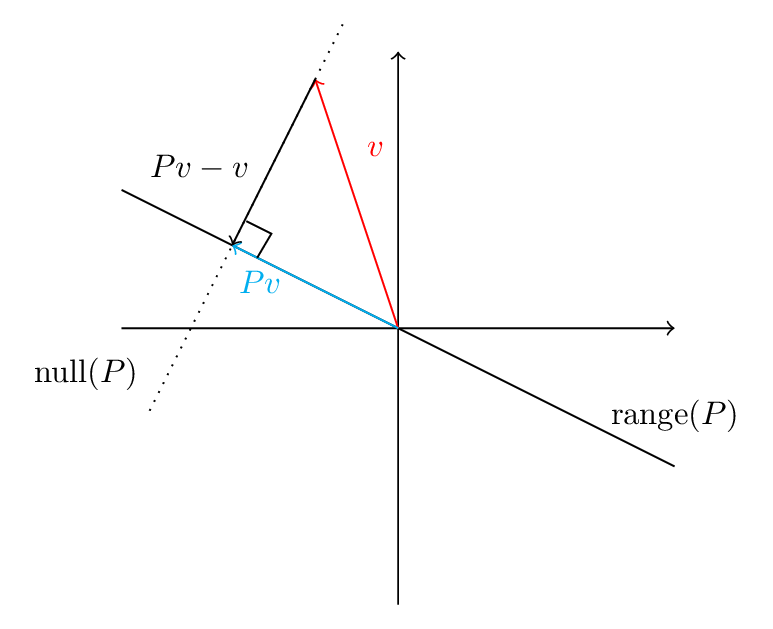
\includegraphics[width=0.6\textwidth]{imgs/orthogonal_proj.png}
%     \caption{Projecting $v$ with Orthogonal Projector $P$}
%     \label{orthogproj}
%   \end{figure}

% \noindent We could see the projector $P$ splits $v$ into two components,  $Pv$ and  $Pv - v$. However, in this case these two components are orthogonal to each other, and computationally, their inner product should be 0. That's where the definition of  \textbf{orthogonal} projector comes from. 

% \noindent \textbf{Note:} More specifically, an orthogonal projector splits $\mathbb{C}^{m}$ into two orthogonal subspaces, range$(P)$ and null$(P)$.

% \bigskip
% \noindent Now we know the definition of an orthogonal projector, but how do we construct an orthogonal projector? \textbf{In this course, we are introduced to construct from a set of orthonormal vectors.} 
% \begin{itemize}
% \item From the knowledge we get in \href{https://comp-lin-alg.github.io/L1_preliminaries.html#constructing-orthogonal-projectors-from-sets-of-orthonormal-vectors}{section 1.10} master notes, we know that, given we have a set of orthonormal vectors $\{q_1, q_2, \ldots, q_n\}$, for all vector $v \in \mathbb{C}^{m}$, we could write $v$ in terms of:
%   \[
%     v = r + \sum_{i = 1}^{n} (q_iq_i^{*})v
%   .\] 
% \item And if we write matrix $\hat{Q}$ as:
%   \[
%     \hat{Q} = \begin{pmatrix} q_1 & q_2 & \ldots & q_n \end{pmatrix} 
%   .\]
%   we could see $\sum_{i=1}^{n} (q_iq_i^{*})v$ is in the column space of $\hat{Q}$, and the component $r$ in $v$ should be orthogonal to any vectors in the orthonormal set $ \{q_i\} $, i.e. $r$ should be orthogonal to the column space of $\hat{Q}$.
%   \item So if we consider $P = \sum_{i=1}^{n} (q_iq_i^{*})$, then we have:
%     \[
%     v = r + Pv
%     .\] 
%     and $r$ and $Pv$ should be orthogonal to each other, as we stated above. So in this case, we have $P$ as our orthogonal projector.
% \end{itemize}
% So now we know how to construct an orthogonal projector, but what the form of an orthogonal projector usually looks like?
% \[
% P \text{ orthogonal } \implies P = \hat{Q}\hat{Q}^{*}
% .\] 
% \subsubsection*{Proof}%
% \begin{itemize}
% \item First of all, computationally if we expand the multiplication $\hat{Q}\hat{Q}^{*}$ :
%   \[
%     \hat{Q}\hat{Q}^* = \begin{pmatrix} q_1 & q_2 & \ldots & q_n \end{pmatrix} \begin{pmatrix} q_1^{*}\\ q_2^{*} \\\vdots\\ q_n^{*} \end{pmatrix} = q_1q_1^* + q_2q_2^* + \ldots + q_nq_n^{*} =  \sum_{i=1}^{n} (q_iq_i^{*})
%   .\]
%   which is exactly what we see in the construction of the orthogonal projector $P$. \textbf{Personally I think all of you should understand the proof at this level.}
% \item Also, in the light of change of basis, the product $\hat{Q}^*v$ gives the coefficients of $v$ after projecting along the columns of  $\hat{Q}$, and the multiplication of $\hat{Q}$ on $\hat{Q}^*v$ gives the projections of $v$ expanded in the canonical basis. 
%   \item Therefore, the multiplication by $\hat{Q}\hat{Q}^*$ does the same job as the orthogonal projector $P$ does. We could finally confirm that the orthogonal projectors has a simple form  $P  = \hat{Q}\hat{Q}^{*}$. 
%   \item \textbf{Note:} the last two parts of the proof are mentioned under \textbf{Theorem 1.28 master notes}, and I think it is not necessary to memory by heart but would give you a deeper understanding if digest them.
% \end{itemize}
% Since any orthogonal projector has the form $P = \hat{Q}\hat{Q}^*$, we have the following properties of orthogonal projectors to discuss:
% \subsubsection*{Property 1}%

% \begin{itemize}
% \item We have known that the orthogonal projector $P$ gives an orthogonal projection to range of $P$. 
% \item However, from our interpretation in the previous proof, the orthogonal projector $\hat{Q}\hat{Q}^*$ would eventually expands any $v$ by columns of $\hat{Q}$. 
% \item So we could conclude that, $P = \hat{Q}\hat{Q}^*$ is an orthogonal projection to range of $\hat{Q}$.
% \item Moreover we could say $\text{range}(P) = \text{range}(\hat{Q})$, since the orthogonal projection on these two planes are equivalent.
% \end{itemize}
% \subsubsection*{Property 2}%
% \begin{itemize}
% \item Similarly, the complementary projector $P_{\bot} = I - \hat{Q}\hat{Q}^*$ would give a orthogonal projection to nullspace of $\hat{Q}$.
% \item And clearly $\text{null}(P) = \text{null}(\hat{Q})$.
% \end{itemize}
% \subsubsection*{Property 3}%
% \begin{itemize}
%   \item Given that any orthogonal projector has the form $P = \hat{Q}\hat{Q}^*$, we could see its adjoint $P^* = (\hat{Q}\hat{Q}^*)^* = (\hat{Q}^*)^*(\hat{Q})^* = \hat{Q}\hat{Q}^* = P$. 
%   \item And we have the following theorem:
%     \[
%     P^* = P \iff P  \text{ orthogonal}
%     .\] 
% \end{itemize}
% \subsubsection*{Proof}%
% \begin{itemize}
% \item The proof of the backward proposition has been shown above, and we need to prove the forward one: $P^* = P \implies P$ orthogonal.
% \item We choose a vector $v \in \mathbb{C}^{m}$ arbitrarily, and we have:
%   \[
%     (Pv)^{*}(Pv - v) = v^*P^*(P - I)v = v^*P(P - I)v 
%   \]
%   \[
%   = v^*(P^2 - P)v = v^*(P - P)v = 0 
%   .\] 
%   Therefore $P$ is orthogonal.
% \end{itemize}

% \subsection*{Exercise 1.30 Constructing Orthogonal Projectors}
% \addcontentsline{toc}{subsection}{Exercise 1.30 Constructing Orthogonal Projectors}
% \subsubsection*{Problem Description}%
% This exercise is a relatively easy one - given an orthonormal set of vectors $Q$, we need to implement a function \href{https://comp-lin-alg.github.io/cla_utils.html#cla_utils.exercises2.orthog_proj}{\texttt{exercises2.orthog\_proj()}} to compute an orthogonal projector $P$, which projects vectors to the subspace spanned by elements of  $Q$.
% \subsubsection*{What to do}%
% We just need to use the construction of orthogonal projector $P = \hat{Q}\hat{Q}^*$, and in this exercise we can easily use our provided $Q$ as the orthonormal matrix. The code implementation should be straightforward enough. \medskip

% \noindent \textbf{Remember to check your implementation pass the provided test cases.}
% \subsubsection*{What happens next}%
% \noindent After learning all the basic things in this chapter, the exited things finally would come in the following chapters \ldots! Next chapter would be based on the knowledge of orthogonal projectors and we would talk about \textbf{QR factorisation}. 

% \bigskip

% \begin{center}
%   \textit{\large \st{End of Week 1 (we haven't finish this week yet!)}} \\
%   \medskip
%   \textit{\large End of Chapter 1}
% \end{center}






\chapter{QR Factorisation}
In computational linear algebra, we would spend a lot of time in matrix equations or expressions like $Ax = b$. However, for large matrices  $A$, it is always difficult and inefficient to find the value of $x$, if we try finding the inverse of $A$ directly. So what we want to do is to "transform" our $A$ into smaller building blocks with specific properties, and use their properties of them to make the equation easier to solve. 

\medskip
\noindent The transformations, should preserve the correctness in matrix calculations (be sufficiently free from truncation errors, as said in the \href{https://comp-lin-alg.github.io/L2_QR_factorisation.html#what-is-the-qr-factorisation}{\textbf{Introduction}} of Chapter 2), and be efficient enough to perform. Here, let us talk about the very first transformation, the \textbf{QR Factorisation}. 
\medskip

\noindent You might have seen this in your year 2 \href{https://github.com/Imperial-MATH50003/MATH50003NumericalAnalysis}{Numerical Analysis} Course, and make some progress in implementation using Julia or Python. We would do some recap and dig further into algorithm stability, and/or time complexities with different ways of implementations.
\newpage
\section{QR Factorisation Concept}%
\begin{definition}[Complete QR Factorisation]
  The \textbf{Complete QR Factorisation} is defined as the processing of decomposing an arbitrary matrix $A \in \mathbb{C}^{m \times  n}$ to the form
  \[
    A = QR \text{ where } Q \text{ unitary } \in \mathbb{C}^{m \times m}, R  \text{ upper triangular } \in \mathbb{C}^{m \times n}
  .\]
\end{definition}
Without loss of generality we consider $m > n$, and have:
\[
\underset{\begin{array}{c}\\ A \end{array}}%
{
\begin{pmatrix}
  a_{11} & a_{12} & \ldots & a_{1n} \\
  a_{21} & a_{22} & \ldots & a_{2n} \\
  \vdots & \vdots & \ddots & \vdots \\
  a_{m1} & a_{m2} & \ldots & a_{mn}
\end{pmatrix}
}
=
\underset{\begin{array}{c}\\ Q \end{array}}%
{
\begin{pmatrix}
  q_{11} & \ldots & q_{1n} & \ldots & q_{1m} \\
  q_{21} & \ldots & q_{2n} & \ldots & q_{2m}\\
  \vdots & \ddots & \vdots & \ddots & \vdots\\
  q_{m1} & \ldots & q_{mn} & \ldots & q_{mm}
\end{pmatrix}
}
\begin{spmatrix}{R}
  r_{11} & r_{12} & \ldots & r_{1n} \\
  0 & r_{22} & \ldots & r_{2n} \\
  0 & 0 & \ldots & r_{3n} \\
  \vdots & \vdots & \ddots & \vdots \\
  0 & 0 & \ldots & r_{nn} \\
  \vdots & \vdots & \ddots & \vdots \\
  0 & 0 & \ldots & 0
\end{spmatrix}
\]
Note that, the term $q_{ik}r_{kj}$ would always give out 0 when $k > n$ and make no contribution to the value of  $a_{ij}$. Therefore, we could only consider the first $n$ columns of $Q$ and the first $n$ rows of $R$ as the result of factorisation.

\begin{definition}[Reduced QR Factorisation]
  The \textbf{Reduced QR Factorisation} is defined as the processing of decomposing an arbitrary matrix $A \in \mathbb{C}^{m \times  n}$ to the form
  \[
    A = \hat{Q}\hat{R} \text{ where } \hat{Q} \text{ unitary } \in \mathbb{C}^{m \times n}, \hat{R}  \text{ upper triangular } \in \mathbb{C}^{n \times n}
  .\]
  where \(\hat{Q}\), \(\hat{R}\) are sub-matrices of the  complete factorisation results \(Q\), \(R\).
\end{definition}
We are mainly talking about the \textbf{reduced} case of QR factorisation in this chapter, but do think about the complete case when doing exercises.

\subsection*{Exercise 2.3: Find an orthonormal basis of the orthogonal complement of a subspace}
\addcontentsline{toc}{subsection}{Exercise 2.3: Find an orthonormal basis of the orthogonal complement of a subspace}
\subsubsection*{Problem Description}%
\label{ssub:problem_description}

Given a set of vectors $ \{v_1, v_2, \ldots, v_n\}$ spans subspace $U \subset \mathbb{C}^{m}$, we need to find an orthonormal basis of its orthogonal complement $U^{\bot}$, defined as:
\[
U^{\bot} = \{x \in \mathbb{C}^{m}: \forall u \in U, x^{*}u = 0\} 
.\] 
Implement this as a function \href{https://comp-lin-alg.github.io/cla_utils.html#cla_utils.exercises2.orthog_space}{\texttt{exercises2.orthog\_space()}}. \medskip

\subsubsection*{Hints}
\begin{enumerate}
  \item Consider the condition \(\forall u \in U, x^{*}u = 0\), can we consider the elements in a smaller \textbf{subset of \(U\)} rather than all elements in \(U\) to simplify the satisfying criteria? If so, what is the subset?
  \item You might find the matrix \(Q\), \(R\) from complete factorisation useful for answering the question above.    
  \item Consider the matrix \(Q\) obtained from the \textbf{complete QR factorisation}, what is the relationship between any two columns of \(Q\)?  
  \item You might want to use the numpy-based QR factorisation routine \texttt{numpy.linalg.qr()}.
\end{enumerate}
If you have the answer to the questions above, you have already got the key to solving this problem. Pause here for a moment to think about how to obtain the orthonormal basis of \(U^{\bot}\). Feel free to read my explanation on the next page if you get confused. \medskip

\noindent \textbf{Remember to check your implementation passes the provided test cases.}
\newpage

\subsubsection*{Spoil Alert \ldots There is a way you could figure out the problem:}%
\begin{itemize}
\item The first thing we need to figure out is, we are finding the vectors that are \textbf{orthogonal to the basis} of \(U\). This could be obtained by the first \(n\) columns in matrix \(Q\) from the complete QR of \(U\).
\item Then we consider the matrix \(Q\). Given that $Q$ is unitary, we would see all column vectors are orthogonal to each other by expanding
  \[
    [Q^*Q]_{ij} = q_i^*q_j = \delta_{ij} = \left\{
      \begin{array}{l}
      0 \text{ when $i \neq j$} \\
      1 \text{ when $i = j$}
      \end{array}
    \right.
  .\] 
  \item We need to find the vectors that are orthogonal to the first \(n\)  column vectors in $Q$, i.e. columns of \(\hat{Q}\). And we could see the remaining $m - n$ columns in  $Q$ are indeed orthogonal to any vector in the first n columns, by the mutual orthogonality mentioned above. 
  \item Therefore, what we need to do is just to find the \textbf{last} $m - n$ \textbf{columns} from $Q$, which should should be the basis of the orthogonal complementary $U^{\bot}$. \checked
\end{itemize}

\newpage
\section{QR Factorisation by Classical Gram-Schmidt}%
We have already seen the concept of QR factorisation, and one of the applications through the previous exercise. Then we are going to explore what exactly happens in this factorisation, via algorithms. The first implementation we would discuss would be the \textbf{classical Gram-Schmidt algorithm}. The algorithm itself is straightforward:
\begin{algorithm}
  \caption{Classical Gram-Schmidt Algorithm}
  \begin{algorithmic}[1]
  \Procedure{GS\_classical}{A}
    \State initialise \(Q, R\)  as empty matrices
    \For{ \(j = 1\) to \(n\)}
      \State \(v_j = a_j\)
      \For{ \(i = 1\) to \(j - 1\)}
        \State \(r_{ij} = q_i^{*}a_j\)
        \State \(v_j = v_j - r_{ij}q_i\)
        \Comment{Remove components of existing \(q_i\) from \(v_j\)}
      \EndFor
      \State \(r_{jj} = \|v_j\|\)  
      \State \(q_j = \frac{v_j}{\|v_j\|}\)
      \Comment{Finish constructing a new basis vector \(q_j\)}
    \EndFor
    \State \Return \(Q, R\)
  \EndProcedure
  \end{algorithmic}
\end{algorithm}

\noindent However, the algorithm might look no sense at all since we haven't discussed the maths behind it so far. Here we look backwards to see how vectors $ \{a_i\} $ factorised to orthonormal vectors $ \{q_i\} $. \medskip

\noindent Just expand $A = QR$ by arithmetic:

 \[
   A = QR \implies \begin{pmatrix} a_1 & a_2 & \ldots & a_n \end{pmatrix} = 
   \begin{pmatrix} 
     q_1 & q_2 & \ldots & q_n 
  \end{pmatrix} 
   \begin{pmatrix} 
     r_{11} & r_{12} & \ldots & r_{1n} \\ 
     0 & r_{22} & \ldots & r_{2n} \\
     \vdots & \vdots & \ddots & \vdots \\
     0 & 0 & \ldots & r_{nn}
   \end{pmatrix}  
.\] 
So we could see the value of any column vector $a_j$ via column-space interpretation and get:
\[
  a_j = 
   \begin{pmatrix} 
     q_1 & q_2 & \ldots & q_j & \ldots & q_n 
  \end{pmatrix} 
  \begin{pmatrix} r_{1j}\\ r_{2j} \\ \vdots\\ r_{jj} \\ 0 \\ \vdots \\ 0 \end{pmatrix}
\] 
\[
  = r_{1j} q_1 + r_{2j}q_2 + r_{3j}q_3 + \ldots + r_{jj}q_j + 0 \cdot q_{j + 1} + \ldots + 0
  = \sum_{i=1}^{j} r_{ij}q_i
.\] 
Starting with $a_1$, we could see that:
 \[
a_1 = r_{11} q_1
.\] 
and in this expression we could observe $q_1$ is the unit vector parallel to $a_1$, so $r_{11}$ and $q_1$ should have the value
\[
r_{11} = \|a_1\| \text{ and } q_1 = \frac{a_1}{\|a_1\|} = \frac{a_1}{r_{11}}
.\]
Then consider $a_2$ from the summation expression above:
 \[
a_2 = r_{12}q_1 + r_{22}q_2
.\]
But we don't know how to get the value of $r_{12}$ yet. Since we know $a_2 = r_{22}q_2 + r_{12}q_1$, and here is the trick to find \(r_{12}\) by using \(q_1\)  :
\[
  q_1^* a_2 = r_{22}(q_1^{*}q_2) + r_{12}(q_1^{*}q_1) = r_{22} \cdot 0 + r_{12} \cdot 1 = r_{12}
.\]
and to get the value of $q_2$ and $r_{22}$, we remove the component of $q_1$ from $a_2$ and we could get:
\[
    v_2 = a_2 - r_{12}q_1 = r_{22}q_2 \implies 
    \left\{
      \begin{array}{l}
      r_{22} = \|v_2\| \\
      q_2 = \frac{v_2}{\|v_2\|} = \frac{v_2}{r_{22}}
      \end{array}
    \right.
.\]
Then we should have an orthonormal set $ \{q_1, q_2\} $, and we could compute corresponding $q_3$ and scale factor $r_{i3}$s in a similar approach. \medskip

\noindent As we repeat these steps iteratively, we could compute the value of $q_4, q_5, \ldots$ until $q_n$, and also the coefficients \(r_{ij}\). And more generally, given matrix \(A \in \mathbb{C}^{m \times n}\), we could compute the entries of \(Q \in \mathbb{C}^{m \times  n}, R \in \mathbb{C}^{n \times  n}\) with the following formula:
\[
  q_j = \frac{v_{j}}{\|v_{j}\|}
\]
\[
  r_{ij} = \left\{
    \begin{array}{ll}
    q_{i}^{*}a_{j} & i < j\\
    \|v_{j}\| & i = j\\
    0 & \text{otherwise}
    \end{array}
  \right.
  \]
  where
  \[
    v_{j} = \left\{
      \begin{array}{ll}
        a_{j} & i = 1\\
        a_{j} - \sum_{k=1}^{j - 1} r_{kj}q_{k} = a_{j} - \sum_{k=1}^{j - 1} (q_{k}q_{k}^{*})a_{j} & \text{otherwise}
      \end{array}
      \right.
      \]
      Now the algorithm above should be easy for you to understand. \checked

\noindent \textbf{Important! Please make sure you understand the gist behind the contents below.}  The expressions of \(r_{ij}\) and \(v_j\) look messy and complex to implement in python. Here we have a concise and elegant way to find the values of \(r_{ij}\) and \(v_j\) via matrix products.
\[
  r_j = \begin{pmatrix} r_j^{(j - 1)} \\ r_{jj} \\ 0 \\ \vdots \\ 0\end{pmatrix} = \begin{pmatrix} Q_{(j - 1)}^{*}a_j \\ \|v_j\| \\ 0 \\ \vdots \\ 0\end{pmatrix}
  \]
  where \(Q_{j - 1} = \begin{pmatrix} 
  q_1 & \dots & q_{j - 1} 
\end{pmatrix} \) and \(r_j^{(j - 1)} = \begin{pmatrix} 
  r_{1j} & \dots & r_{(j-1)j}
\end{pmatrix} \), with   
\[
  v_j = a_j - Q_{j - 1}r_j^{(j - 1)} = a_j - Q_{j - 1}(Q_{j - 1}^{*}a_j) = (I - Q_{j - 1}Q_{j - 1}^{*})a_j
\]
Note that the \(^{*}\) here \textbf{refers to the adjoint of a matrix}, not the scalar multiplication!
\textbf{Do pause here for a while to make sure you could show the expressions above by yourself.} \medskip

\noindent 
You can see we are now eliminating the index \(i\) in every expression by replacing the summation with matrix products. This is essential since you can get rid of one for-loop with variable \(i\)  in the algorithm above, and use NumPy-based matrix multiplication. \smallskip

\noindent Since we've seen the fact that using matmul in NumPy is more efficient than using for loops, you should pay more attention to using more "vectorized operations" like matmul, and \textbf{reduce for loops as much as possible. }

\noindent Here is the optimised version of the classical Gram-Schmidt algorithm, \textbf{which is not mentioned by the lecturer} but you would \textbf{lose marks if not optimised.}
\begin{algorithm}
  \caption{Classical Gram-Schmidt Algorithm, optimised}
  \begin{algorithmic}[1]
  \Procedure{GS\_classical\_optimised}{A}
    \State initialise \(Q, R\)  as empty matrices
    \For{ \(j = 1\) to \(n\)}
      \State \(r_j^{(j - 1)} = Q_{(j - 1)}^{*}a_j\)
      \State \(v_j = a_j - Q_{j - 1}r_j^{(j - 1)}\)
      \State \(r_{jj} = \|v_j\|\)
      \State \(q_j = \frac{v_j}{\|r_{jj}\|}\)    
    \EndFor
    \State \Return \(Q, R\) 
  \EndProcedure
  \end{algorithmic}
\end{algorithm}

\newpage
\noindent To let you have a more direct sense of classical Gram-Schmidt, \autoref{cgs} would demonstrate the flow of the classical Gram-Schmidt Algorithm. 
\begin{figure}[htp]
  \centering
  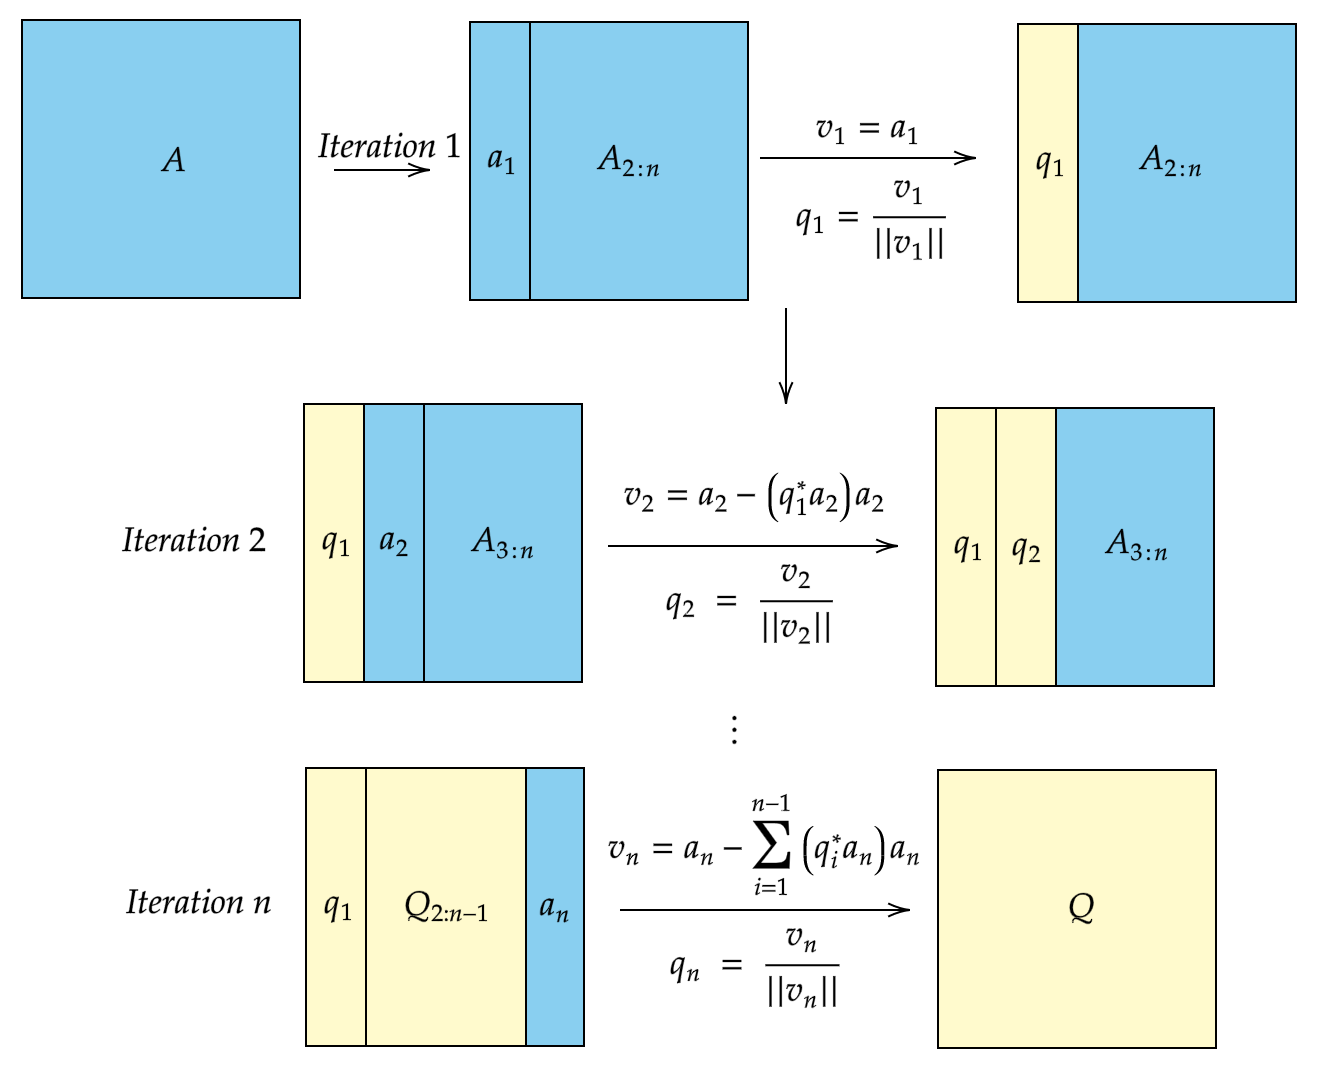
\includegraphics[width=\textwidth]{imgs/cgs.png}
  \caption{Classical Gram-Schmidt Algorithm Demonstration}
  \label{cgs}
\end{figure}

\noindent The only difference between the algorithm and \autoref{cgs} is I didn't create another array to store column-vectors of \(Q\) but in the sense of "converting" \(A\)  to \(Q\)  column-wise.
\newpage
\subsection*{Exercise 2.4: Implement the Classical Gram-Schmidt Algorithm}
\addcontentsline{toc}{subsection}{Exercise 2.4: Implement the Classical Gram-Schmidt Algorithm}
\subsubsection*{Problem Description}%
Here you need to implement the classical Gram-Schmidt algorithm from the derivation above in your function \href{https://comp-lin-alg.github.io/cla_utils.html#cla_utils.exercises2.GS_classical}{\texttt{exercises2.GS\_classical()}}. Note that instead returning matrices \(Q\) and \(R\) from the function, you need to change original matrix \(A\) to \(Q\) 'in-place' (which is in the way I demonstrated in \autoref{cgs}) and return \(R\) only.
\subsubsection*{What to do}
There is not too much to talk about in this exercise. However, two things are still worth mentioning:
\begin{enumerate}
  \item You are asked to change \(A\)  to \(Q\)  "in-place", which is not mentioned in the pseudo-code above. A good initiative to achieve this is to initialise \texttt{Q = A} in your function and follow the optimised algorithm to write your code. 
  \item When creating empty or zero matrices with NumPy, the matrices would not be initialised as complex matrices. You might find specifying \texttt{dtype=np.complex128} or \texttt{dtype=A.dtype} useful in your code implementation.  
\end{enumerate}
The main task for you now is to not be confused between indexes in maths formulas and Python (starting from 0). Try using 'vectorized' operations in your implementation, e.g. matrix multiplication rather than additional loops. \medskip

\noindent \textbf{Remember to check your implementation passes the provided test cases.}

\section{QR Factorisation by Modified Gram-Schmidt}
This part is the modification of classical Gram-Schmidt and contains two coding exercises. The initiative we want to make a modified version of classical Gram-Schmidt is due to the instability of classical GS. Here is the demonstration:\medskip

\noindent Let us say we have obtained \(Q, R\) from classical Gram-Schmidt, and mathematically we should have \(QR = A\). But since there are lots of rounding errors from the inexact arithmetic when this algorithm runs on computers, the entries of \(Q, R\)  are "polluted" so it is not necessarily correct for the equation \(QR = A\) when we do factorisation with classical GS. \medskip

\noindent Therefore the mathematicians propose a quick fix to the classical GS algorithm, and we called the modified version as \textbf{modified Gram-Schmidt}. The algorithm goes in this way:

\begin{algorithm}
\caption{Modified Gram-Schmidt Algorithm}
\label{mgs-algorithm}
\begin{algorithmic}[1]
\Procedure{GS\_modified}{A}
  \State initialise \(Q, R\)  as empty matrices
  \For{ \(i = 1\) to \(n\)}
    \State \(v_i = a_i\)
    \State \(r_{ii} = \frac{v_i}{\|v_i\|}\)  
    \For{ \(j = i + 1\) to \(n\)}
      \State \(r_{ij} = q_i^{*}v_j\)
      \State \(v_j = v_j - r_{ij}q_i\)
      \Comment{Remove components of \(q_i\) from all \(v_j\)s}
    \EndFor
    \Comment{Finish constructing a new basis vector \(q_j\)}
  \EndFor
  \State \Return \(Q, R\)
\EndProcedure
\end{algorithmic}
\end{algorithm}

\noindent To let you have a more direct sense of modified Gram-Schmidt, \autoref{mgs} would demonstrate the flow of the modified Gram-Schmidt Algorithm. \medskip
\begin{figure}[H]
  \centering
  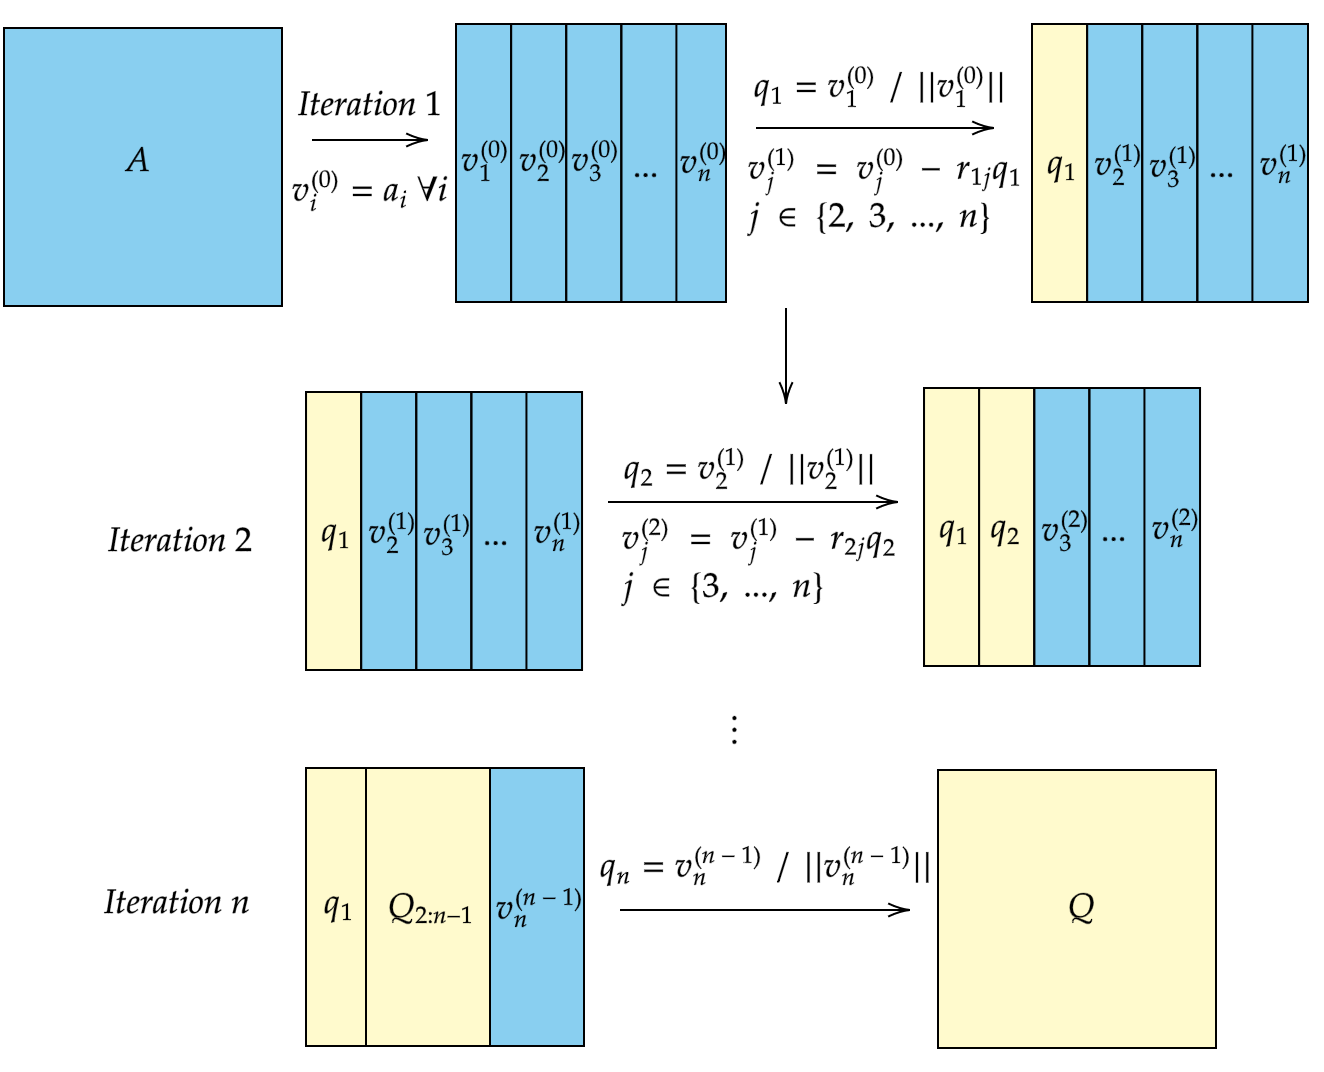
\includegraphics[width=0.9\textwidth]{imgs/mgs.png}
  \caption{Modified Gram-Schmidt Algorithm Demonstration}
  \label{mgs}
\end{figure}
\noindent You might find it confusing that, there are also superscripts in \(v_k\)  in \autoref{mgs} above, e.g. \(v_3^{(2)}\). The notation \(v_k^{(i)}\)  here is just for demonstrating the updated value of column vector \(v_k\) after iteration \(i\). 

\noindent For simplicity, I will ignore the superscripts \(^{(i)}\) in \(v_k\) in the following explanations, and I hope you could still understand the upcoming contents. \medskip

\noindent Essentially the modified GS and the classical GS have the same effect in factorisation. Recall that in classical GS what we did in each iteration \(k\) is, \textbf{set the vector \(v_k = a_k\), remove the components of found \(\{q_1, q_2, ..., q_{k - 1}\}\) from \(v_k\), set the normalised (and updated) \(v_k\) as \(q_k\), and add the obtained \(q_k\)  to the existing orthonormal set \(\{q_i\}\)} for the next iteration. However, what we did in the modified GS is, for each iteration \(k\), \textbf{I picked up the column vector \(v_k\), normalise it to obtain a basis vector \(q_k\), and remove the components of \(q_k\) from the vectors \(\{v_{k + 1}, ..., v_{n}\}\)} behind. \medskip

\noindent The two algorithms indeed have the same effect on an arbitrary matrix \(A\), and also have the same number of computational operations. However, the main difference is that in modified GS we define \(r_{ij} = q_i^{*}v_j\) rather than \(r_{ij} = q_i^{*}a_j\). In this case, \textbf{the rounding error} in finding \(r_{ij}\) would be \textbf{smaller} and the \textbf{algorithm will be more stable.} Click \href{https://math.stackexchange.com/questions/3913710/intuitive-explanation-of-why-the-modified-gram-schmidt-is-more-stable-than-the-c}{here} to see the explanation.\medskip

\noindent You might think now you should be ready for implementing this algorithm by yourself. However, from one of the gist in this course, \textbf{you should use avoid "additional" for loops as much as possible}. That is to say, you should consider if you could reduce the number of "for loops" in the algorithm shown in the class/on the website. Pause here for a while to think about it, and go to the next page for checking my solution to reduce no. of for-loops by introducing vectorized operations. 

\newpage
\noindent Consider the inner for-loop starting from \textbf{line 6 to line 9} in \autoref{mgs-algorithm}. Firstly we should see in this loop we computed the values \(\{r_{i(i + 1)}, r_{i(i + 2)}, ..., r_n\}\), by arithmetic we should see
\[
  r_i^{(i + 1, n)} = \begin{pmatrix} 
    r_{i(i + 1)} \\ r_{i(i + 2)} \\ \vdots \\ r_n
  \end{pmatrix}
  = 
  \begin{pmatrix} 
      q_i^{*}v_{i + 1} \\
      q_i^{*}v_{i + 2} \\
      \vdots \\
      q_i^{*}v_{n}
  \end{pmatrix}
  = \begin{pmatrix} 
     v_{i + 1}^{*}q_i & v_{i + 2}^{*}q_i & ... & v_{n}^{*}q_i
  \end{pmatrix}^{*}
\]
\[
  =
  (\begin{pmatrix} 
    v_{i + 1}^{*}q_i \\
    v_{i + 2}^{*}q_i \\
    \vdots \\
    v_{n}^{*}q_i
\end{pmatrix}^{\top})^{*}
  = ((V_{i + 1}^{*}q_i)^{\top})^{*} = ((V_{i + 1}^{*}q_i)^{*})^{\top} 
\]
\[
  = (q_i^{*}V_{i + 1})^{\top} = V_{i + 1}^{\top}\overline{q_i}
\]
where \(V_{i + 1} = \begin{pmatrix} 
    v_{i + 1} & v_{i + 2} & ... & v_{n}
\end{pmatrix} \)  and \(\overline{q_i}\) is the complex conjugate of \(q_i\). \medskip

\noindent Also we could see the component of \(q_i\)  is removed from \(\{v_{i + 1}, v_{i + 2}, ..., v_{n}\} \) in iteration \(i\). Recall the definition of outer product \(uv^{\top}\) and we should see
\[
  V_{i + 1} = V_{i + 1}
  - \begin{pmatrix} 
    r_{i(i + 1)}q_i & r_{i(i + 2)}q_i & ... & r_{in}q_i 
  \end{pmatrix} 
\]
\[
  = V_{i + 1} - q_i \begin{pmatrix} 
    r_{i(i + 1)} \\
    r_{i(i + 2)} \\
    \vdots \\
    r_{in}
  \end{pmatrix}^{\top}
  = V_{i + 1} - q_i (r_i^{(i + 1, n)})^{\top}
\]
Therefore, you now have the optimised version of the modified Gram-Schmidt algorithm, which is not mentioned by the lecturer but you would lose marks if not optimised.

\begin{algorithm}
  \caption{Modified Gram-Schmidt Algorithm, optimised}
  \label{mgs-algorithm-optimised}
  \begin{algorithmic}[1]
  \Procedure{GS\_modified\_optimised}{A}
    \State initialise \(Q, R\)  as empty matrices
    \For{ \(i = 1\) to \(n\)}
      \State \(v_i = a_i\)
      \State \(r_{ii} = \frac{v_i}{\|v_i\|}\)
      \State \(r_i^{(i + 1, n)} = V_{i + 1}^{\top}\overline{q_i}\)
      \State \(V_{i + 1} = V_{i + 1} - \overline{q_i} (r_i^{(i + 1, n)})^{\top}\)    
    \EndFor
    \State \Return \(Q, R\)
  \EndProcedure
  \end{algorithmic}
  \end{algorithm}

\subsection*{Exercise 2.5: Implement the Modified Gram-Schmidt Algorithm}
\addcontentsline{toc}{subsection}{Exercise 2.5: Implement the Modified Gram-Schmidt Algorithm}
\subsubsection*{Problem Description}%
You are now asked to implement the modified Gram-Schmidt algorithm in \href{https://comp-lin-alg.github.io/cla_utils.html#cla_utils.exercises2.GS_modified}{\texttt{exercises2.GS\_modified}}. You should be able to implement it with the minimum amount of loops from reading the optimised algorithm above. \medskip

\noindent \textbf{Remember to check your implementation passes the provided test cases.}

\section{Modified Gram-Schmidt Algorithm with Triangular Orthogonalisation}
From \autoref{mgs} you should see how modified Gram-Schmidt works iteratively. However, from another perspective, we could consider each iteration \(k\) as a transformation represented by matrix \(R_k\). Let us say $\hat{A}_0 = A$ and $\hat{A}_{k} = \hat{A}_{k - 1}R_k$, the transformation \(R_k\) should satisfy the following criteria:
\[
  \hat{A}_0 = \begin{pmatrix} v_{1}^{(0)} & v_{2}^{(0)} & \ldots & v_{n}^{(0)}\end{pmatrix} = A
\] and 
\[
  \hat{A}_{k} = \begin{pmatrix} v_1^{(k)} & v_2^{(k)} & \ldots & v_{n}^{(k)} \end{pmatrix} = \hat{A}_{k - 1}R_{k}
\] 
\begin{enumerate}
  \item The first $k - 1$ columns in $\hat{A}_{k - 1}$ and $\hat{A}_{k}$ should be the same after transformation. i.e. 
  \[
    \begin{pmatrix} v_1^{(k - 1)} & \ldots & v_{k - 1}^{(k - 1)} \end{pmatrix} = \begin{pmatrix} v_1^{(k)} & \ldots & v_{k - 1}^{(k)} \end{pmatrix} 
  \] 
  \item The $k$-th column in $\hat{A}_{k}$ is the normalised vector of column $k$ in $\hat{A}_{k - 1}$. i.e.
    \[
    v_{k}^{(k)} = \frac{v_{k}^{(k - 1)}}{\|v_{k}^{(k - 1)}\|}
    \] 
  \item The last $(n - k)$ columns in $\hat{A}_{k}$ is transformed from $\hat{A}_{k - 1}$ where
    \[
      v_{i}^{(k)} = v_{i}^{(k - 1)} - r_{ki} \frac{v_k^{(k - 1)}}{\|v_{k}^{(k - 1)}\|} = v_{i}^{(k - 1)} - \frac{r_{ki}}{r_{kk}}v_{k}^{(k - 1)} ~\forall i \in \{k + 1, k + 2, \ldots, n\} 
    \] 
    where
    \[
      r_{kk} = \|v_{k}^{(k - 1)}\|, r_{ki} = q_k^{*}v_{i}^{(k - 1)} = \frac{(v_k^{(k - 1)})^{*}v_{i}^{(k - 1)}}{\|v_{k}^{(k - 1)}\|}
    \]  
\end{enumerate}
Recall here we use the notation \(v_l^{(r)}\) for demonstrating the updated value of column vector \(v_l\) after iteration \(r\).
\begin{itemize}
  \item From the \textbf{Criteria 1} we could see that, when $1 \le  l \le  k - 1$, the $l$-th column vector of $\hat{R}_{k}$ should be the base vector $e_{l}$. i.e. the $r$-th element in vector $e_l$ is represented as the Kronecker delta $\delta_{lr}$.
  \item From the \textbf{Criteria 2} we could see that the $k$-th column vector of $ \hat{R}_{k}$ should be $\frac{e_k}{r_{kk}}$ in which $e_k$ follows the same definition as above.
  \item From the  \textbf{Criteria 3} we could see that the last $(n - k)$ columns of $\hat{R}_{k}$ (say the column $i$ is called $r_{k}^{(i)}$) should be in the form
    \[
      [r_{k}^{(i)}]_j = \left\{
        \begin{array}{ccl}
          1 &~ & $j = i$ \\
          -\frac{r_{ki}}{r_{kk}} & ~&$j = k$ \\
          0 & ~&\text{otherwise}
        \end{array}
      \right.
    .\] 
\end{itemize}
Therefore, the matrix $\hat{R}_{k}$ should take the form when $k = 2$:
\[
  \hat{R}_{k} = \begin{pmatrix}
  1 & 0 & 0 & \ldots & 0 \\
  0 & \frac{1}{r_{22}} & -\frac{r_{23}}{r_{22}} & \ldots & -\frac{r_{2n}}{r_{22}} \\
  0 & 0 & 1 & \ldots & 0 \\
  \vdots & \ddots & \ddots & \ddots & \vdots \\
  0 & \ldots & 0 & \ldots & 1
\end{pmatrix} 
\]
i.e. A $n \times n$ identity matrix except row $k$ is filled starting from the diagonal element $r_{kk}$, where the diagonal element is $\frac{1}{r_{kk}}$ and the elements behind the element takes the form $-\frac{r_{ki}}{r_{kk}}$, where $i$ is the column index. In which case
\[
  \{-\frac{r_{ki}}{r_{kk}}\} = \begin{pmatrix} 
    - \frac{r_{k(k + 1)}}{r_{kk}} \\ -\frac{r_{k(k + 1)}}{r_{kk}} \\ \vdots \\ -\frac{r_{kn}}{r_{kk}}
  \end{pmatrix} = -\frac{1}{\|v_{k}^{(k - 1)}\|}\begin{pmatrix} 
    (v_k^{(k - 1)})^{*}v_{k + 1}^{(k - 1)} \\
    (v_k^{(k - 1)})^{*}v_{k + 2}^{(k - 1)} \\
    \vdots \\
    (v_k^{(k - 1)})^{*}v_{n}^{(k - 1)}
  \end{pmatrix} = -\frac{(V_{k + 1}^{(k - 1)})^{\top}\overline{v_k^{(k - 1)}}}{\|v_{k}^{(k - 1)}\|}
\]
where \(V_{k + 1}^{(k - 1)} = \begin{pmatrix} 
  v_{k + 1}^{(k - 1)} & v_{k + 2}^{(k - 1)} & ... & v_{n}^{(k - 1)}
\end{pmatrix} \). i.e. the last \(n - k\) cols of \(\hat{A}_{k - 1}\).  \medskip

\noindent You should also see that inductively the $\hat{Q}$ obtained from this method takes this form:
\[
\hat{Q} = A \hat{R}_1 \hat{R}_2 \ldots \hat{R}_n
\] 
And since every $\hat{R}_k$ is essentially an upper triangular matrix, so do their products. We know that the inverse of an upper triangular matrix is still upper triangular, so we could obtain $\hat{R}$ from the inverse of product $\prod_{k=1}^{n}\hat{R}_k$. \medskip

\noindent Also here we are using a series of \textbf{upper triangular} matrices to obtain an orthogonal matrix $\hat{Q}$, and this is the reason we called it \textbf{triangular orthogonalisation}. The algorithm with triangular orthogonalisation in modified Gram-Schmidt is shown below:

\begin{algorithm}[H]
  \caption{Get \(R_k\) for triangular orthogonalisation in modified GS}
  \label{mgs-get-r}
  \begin{algorithmic}[1]
  \Procedure{GS\_modified\_get\_R}{$\hat{A}_{k - 1}$, $k$} 
    \State initialise \(\hat{R}_k\)  as an identity matrix
    \State \(\hat{R}_{k}\)\texttt{[k, k]} \(= \|\hat{A}_{k - 1}\texttt{[:, k]}\|\)
    \State \(\hat{R}_{k}\)\texttt{[k, k + 1:]} \(=- \frac{\hat{A}_{k - 1}\texttt{[:, k + 1:]}^{\top} \overline{\hat{A}_{k - 1}\texttt{[:, k]}}}{\hat{R}_{k}\texttt{[k, k]}}\)       
    \State \Return \(\hat{R}_k\)
  \EndProcedure
  \end{algorithmic}
  \end{algorithm}
\noindent Note that some implementations of this algorithm will not explicitly mention \(\hat{A}_{k - 1}\) as the input parameter, instead the input parameter would be a general matrix \(A\). Keep this in mind and you might need this in exercise. 
\begin{algorithm}[H]
  \caption{Modified Gram-Schmidt with Triangular Orthogonalisation}
  \label{mgs-r}
  \begin{algorithmic}[1]
  \Procedure{GS\_modified\_R}{$A$} 
    \State \texttt{m, n = A.shape}
    \State initialise \(Q, R\) as \(A\) and an identity matrix
    \For{ \(k = 1\) to \(n\)}
      \State \(\hat{R}_k = \)  GS\_MODIFIED\_GET\_R\((A, k)\)
      \State \(Q = Q \hat{R}_{k}\)
      \State \(R = R \hat{R}_{k}\)     
    \EndFor
    \State \Return \(Q, R\)
  \EndProcedure
  \end{algorithmic}
  \end{algorithm}

  \subsection*{Exercise 2.6: Implement the \texttt{get\_R()} Function Modified GS}
  \addcontentsline{toc}{subsection}{Exercise 2.6: Implement the \texttt{get\_R()} Function Modified GS}
  \subsubsection*{Problem Description}%
  You are now asked to implement the modified Gram-Schmidt algorithm in \href{https://comp-lin-alg.github.io/cla_utils.html#cla_utils.exercises2.GS_modified_get_R}{\texttt{exercises2.GS\_modified\_get\_R}}. You should be able to implement it with reference of \autoref{mgs-get-r}. \medskip
  
\noindent \textbf{Remember to check your implementation passes the provided test cases.}


 \bigskip

 \begin{center}
   \textit{\large End of Week 2}
 \end{center}


% \chapter{Analysing Algorithms}
% \input{chapters/algoana}

% \chapter{LU Decomposition}
% \input{chapters/ludecomp}

% \chapter{Finding Eigenvalues of Matrices}
% \input{chapters/eigenvalues}

% \chapter{Iterative Krylov Methods for $Ax = b$}
% \input{chapters/krylov}
% \appendix
% \chapter{Sample Solution for Programming Exercises}
% I didn't usually give out my code as sample solution. If you could see this part, then you have my greatest trust of making good use of my work. Hope this would help. \medskip

\noindent Here I would not emphasize on the mathematical background behind the code, since they should be mentioned in the hints of each exercise. I would share my comment focusing on writing concise and fluent code to give you some idea of improving code efficiency and readability.

\section{Exercises 1}

\subsection{Implementation of \texttt{basic\_matvec()}}
\lstinputlisting[language=Python, firstline=17, lastline=28]{./python/exercise1.py}
You might notice that, unlike using empty list and initialize \(b_i\) in each loop in the exercise hint, I used \texttt{np.zeros} to initialize an all-zero vector as my initial \(b\), so there is no need to add an extra line to set \(b_i = 0\) and append final calculated \(b_i\) to \(b\). Instead we just update the elements in \(b\) and return it once the loop terminates.
\newpage
\subsection{Implementation of \texttt{column\_matvec()}}
\lstinputlisting[language=Python, firstline=31, lastline=36]{./python/exercise1.py}
You might think using \texttt{for i in range(len(A))} is also correct - indeed, but then you need to get entries of \(x\) via x[i] and the nested brackets with \texttt{range()} and \texttt{len()} are not concise enough for readers.
\medskip

\noindent 
We use \href{https://realpython.com/python-enumerate/}{\texttt{enumerate()}} instead for better readability. If you are not familiar with \texttt{enumerate()}, you can think \texttt{enumerate()} converts a sequence of elements \texttt{\{'a', 'b', \ldots, 'z'\}} (Note: this doesn't mean the sequence is a \texttt{set()} object in python.) 
to a sequence of \texttt{(index, element)} pair \texttt{\{(0, 'a'), (1, 'b'), \ldots, (25, 'z')\}}. \medskip

\noindent Here is an example:
\lstinputlisting[language=Python, firstline=38, lastline=40]{./python/exercise1.py}
And the output would be:
\begin{lstlisting}
0 a
1 b
2 d
3 c
\end{lstlisting}
\subsection{Implementation of \texttt{rank2()}}
\lstinputlisting[language=Python, firstline=43, lastline=50]{./python/exercise1.py}
Don't panic if you see the "@" operator and have no idea about it. This is the matrix multiplication operator introduced since Python 3.5 (I hope you are all able to use this). It is definitely a cool and concise operator and I really recommend you to use this rather than methods like \texttt{matmul()} or \texttt{dot()}.
\newpage
\subsection{Implementation of \texttt{rank1pert\_inv()}}
\lstinputlisting[language=Python, firstline=53, lastline=56]{./python/exercise1.py}
\subsection{Implementation of \texttt{ABiC()}}
\lstinputlisting[language=Python, firstline=80, lastline=97]{./python/exercise1.py}
You might be confused with \texttt{m, \_ = Ahat.shape}, and there is nothing to worry about. Let me show you an example:
\begin{itemize}
    \item Firstly, if \(A\) is a \(m \times  n\) numpy array(or say matrix), when we use \texttt{A.shape}, the code would return a tuple \((m, n)\). And if we want to let \(a = m, b = n\), the naive way is to assign them separately, using:
    \[
    \begin{array}{c}
        \texttt{a = A.shape[0]} \\
        \texttt{b = A.shape[1]}
    \end{array}
    \]
    \item But we could write this in a more elegant way, using:
    \[
        \texttt{a, b = A.shape}
    \]
    where \texttt{A.shape} returns a tuple \(m, n\) and the assignment \texttt{a, b = A.shape} unpack the tuple and assign the values separately in one line.
    \item However, if we only want one dimension e.g. \(m\) and we don't want to bothered with indexing issues (like whether indexing in python starts from 0 or 1), we could use the code style above, and replace the unwanted variable with an \texttt{"\_"}, representing as:
    \[
        \texttt{a, \_ = A.shape}
    \]
\end{itemize}

\section{Exercises 2}
\subsection{Implementation of \texttt{orthog\_cpts()}}
\lstinputlisting[language=Python, firstline=6, lastline=9]{./python/exercise2.py}

\subsection{Implementation of \texttt{solveQ()}}
\lstinputlisting[language=Python, firstline=12, lastline=14]{./python/exercise2.py}

\subsection{Implementation of \texttt{orthog\_proj()}}
\lstinputlisting[language=Python, firstline=34, lastline=35]{./python/exercise2.py}

\end{document}

